\chapter{Fe-Pd Potential}
\label{chapter:appendix-fepdpotential}

This potential has been developed specifically for Fe and Pd where the atoms are in an \acrshort{fcc} structure.  Particular weighting was given to the relaxed configurations of each pure element, those with small additions of Pd to Fe and surface/slab configurations.

\section{Tabulated Potential}

The files for the potential are large, with the \acrshort{lammps} version being over 7,000 lines long containing 35,000+ data points.  They are not included here but are available to download from:

https://github.com/BenPalmer1983/fepd\_feru\_potential



\clearpage
\FloatBarrier
\section{Potential Function Plots}

The seven functions that make up the potential are plotted in figure \ref{fig:fepd-fcc-function-plots}.

\begin{figure}[htb]
\begin{subfigure}{.32\textwidth}
  \centering
  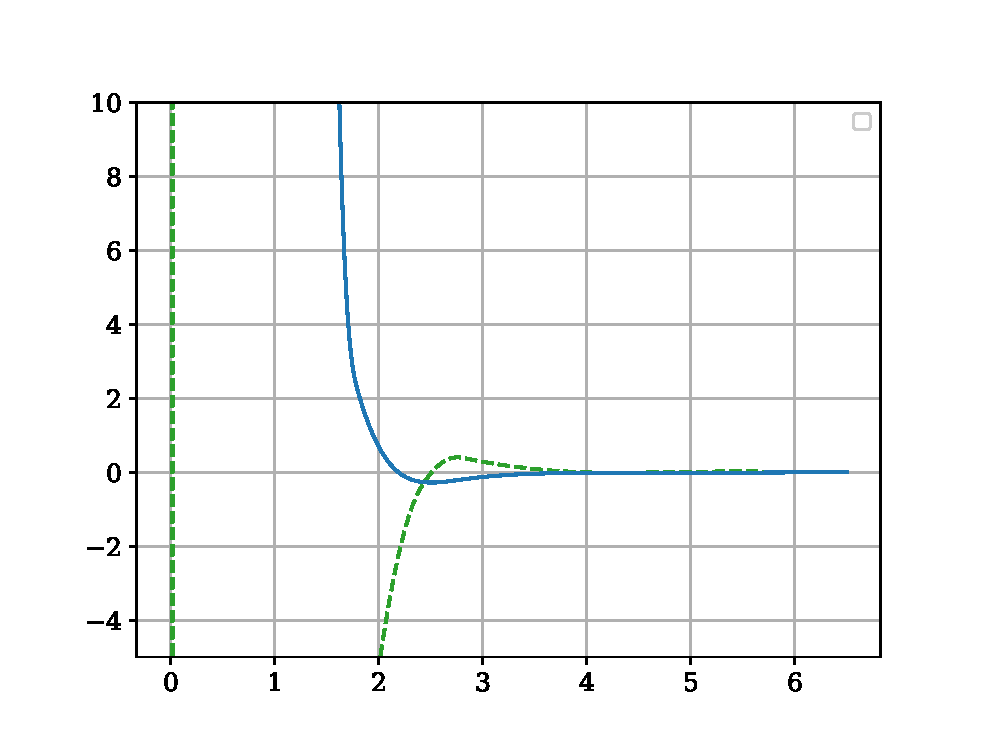
\includegraphics[width=.94\linewidth]{chapters/potentials_fe_pd_ru/fepd_potential/function_plots/fefe_pair.eps}  
  \caption{Fe-Fe Pair}
  \label{fig:fepd-fefe-pair}
\end{subfigure}
\begin{subfigure}{.32\textwidth}
  \centering
  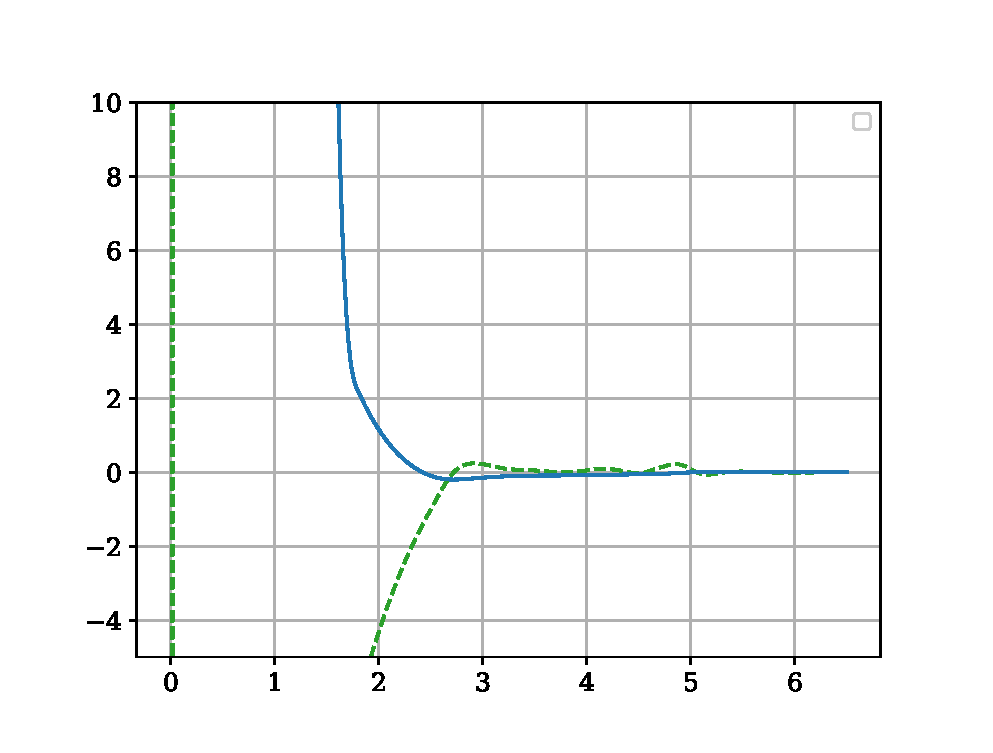
\includegraphics[width=.94\linewidth]{chapters/potentials_fe_pd_ru/fepd_potential/function_plots/fepd_pair.eps}  
  \caption{Fe-Pd Pair}
  \label{fig:fepd-fepd-pair}
\end{subfigure}
\begin{subfigure}{.32\textwidth}
  \centering
  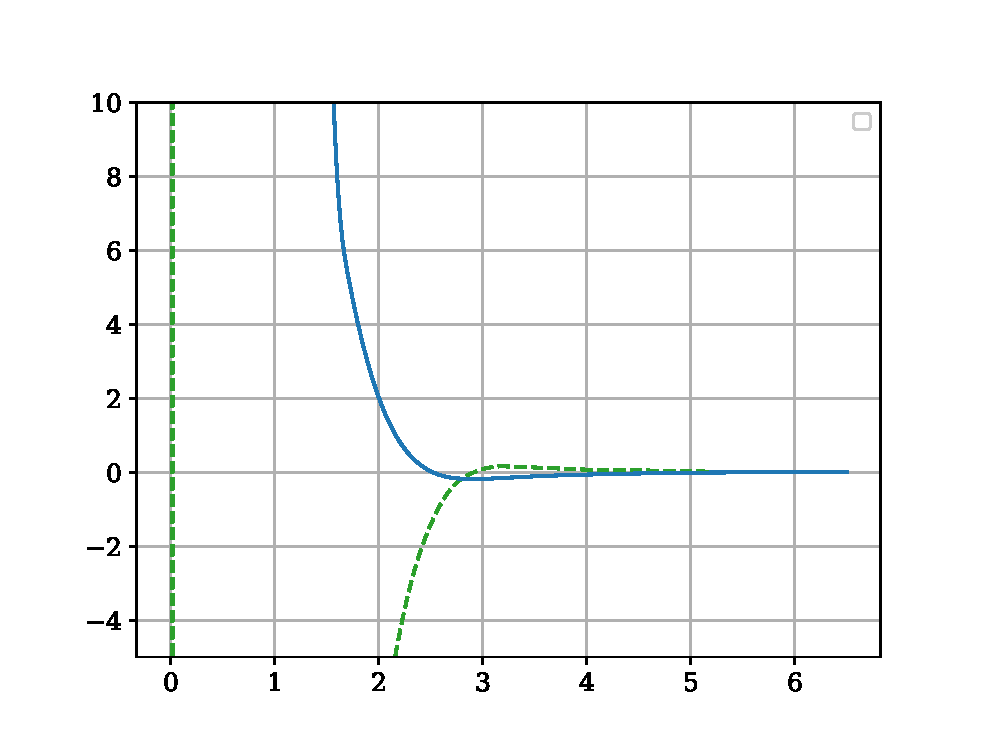
\includegraphics[width=.94\linewidth]{chapters/potentials_fe_pd_ru/fepd_potential/function_plots/pdpd_pair.eps}  
  \caption{Pd-Pd Pair}
  \label{fig:fepd-pdpd-pair}
\end{subfigure}
\begin{subfigure}{.32\textwidth}
  \centering
  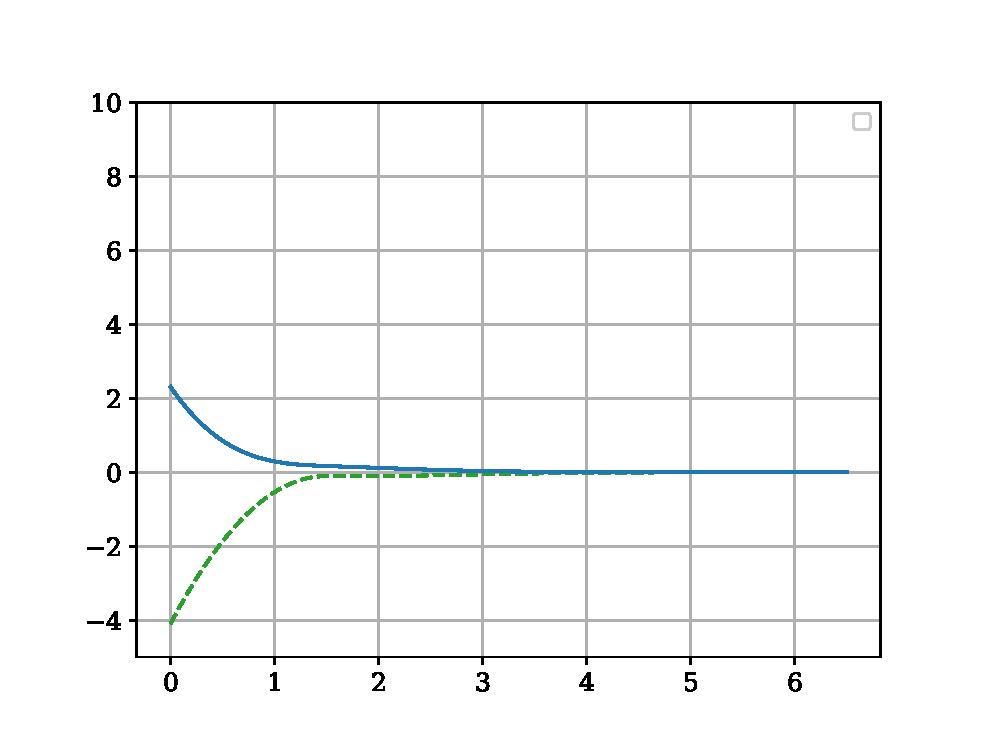
\includegraphics[width=.94\linewidth]{chapters/potentials_fe_pd_ru/fepd_potential/function_plots/fe_dens.eps}  
  \caption{Fe Density}
  \label{fig:fepd-fe-dens}
\end{subfigure}
\begin{subfigure}{.32\textwidth}
  \centering
  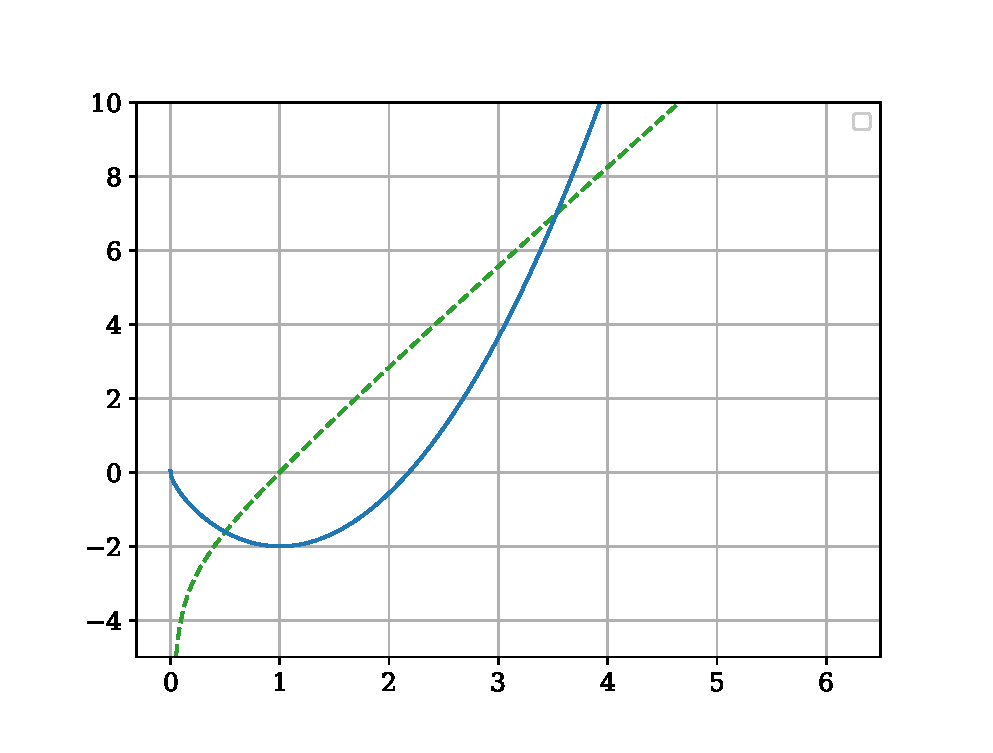
\includegraphics[width=.94\linewidth]{chapters/potentials_fe_pd_ru/fepd_potential/function_plots/fe_embe.eps}  
  \caption{Fe Embed}
  \label{fig:fepd-fe-embe}
\end{subfigure}
\begin{subfigure}{.32\textwidth}
  \centering
  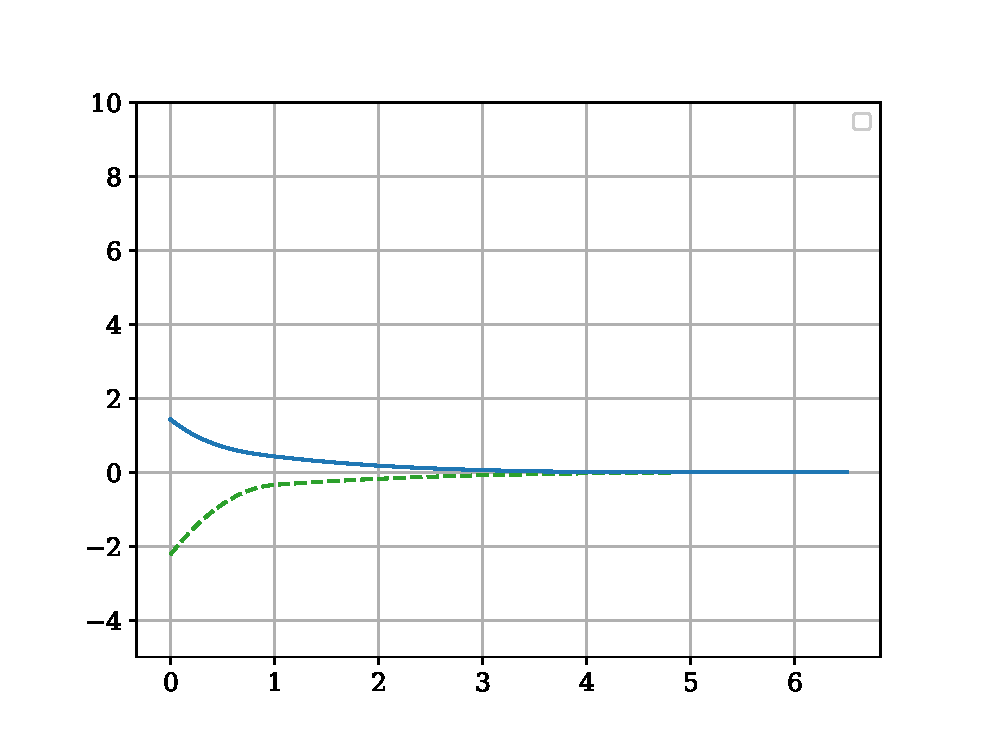
\includegraphics[width=.94\linewidth]{chapters/potentials_fe_pd_ru/fepd_potential/function_plots/pd_dens.eps}  
  \caption{Pd Density}
  \label{fig:fepd-pd-dens}
\end{subfigure}
\begin{subfigure}{.32\textwidth}
  \centering
  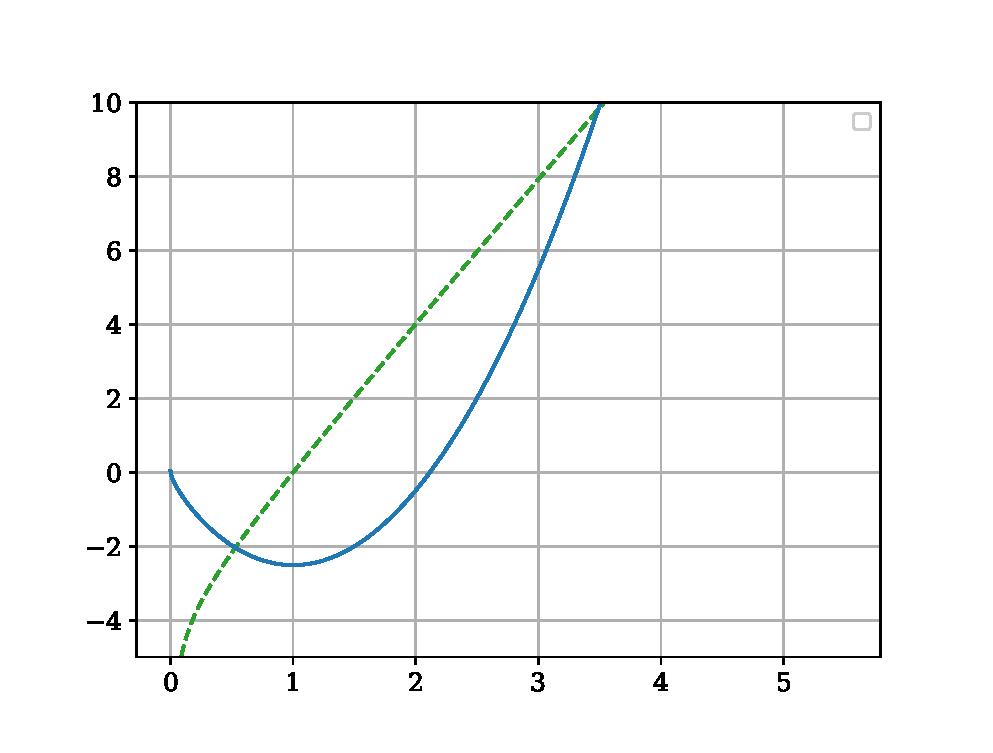
\includegraphics[width=.94\linewidth]{chapters/potentials_fe_pd_ru/fepd_potential/function_plots/pd_embe.eps}  
  \caption{Pd Embed}
  \label{fig:fepd-pd-embe}
\end{subfigure}
\label{fig:fepd-fcc-function-plots}
\caption{Binary Alloy Potential for Fe-Pd}
\end{figure}









\clearpage
\section{Potential vs DFT}

The potentials were derived with a larger weight applied to a smaller set of configurations.  How well the potential fits to the \acrshort{dft} results in terms of energy is given in figure \ref{fig:fepd-energy}.

\begin{figure}[htb]
\begin{subfigure}{.42\textwidth}
  \centering
  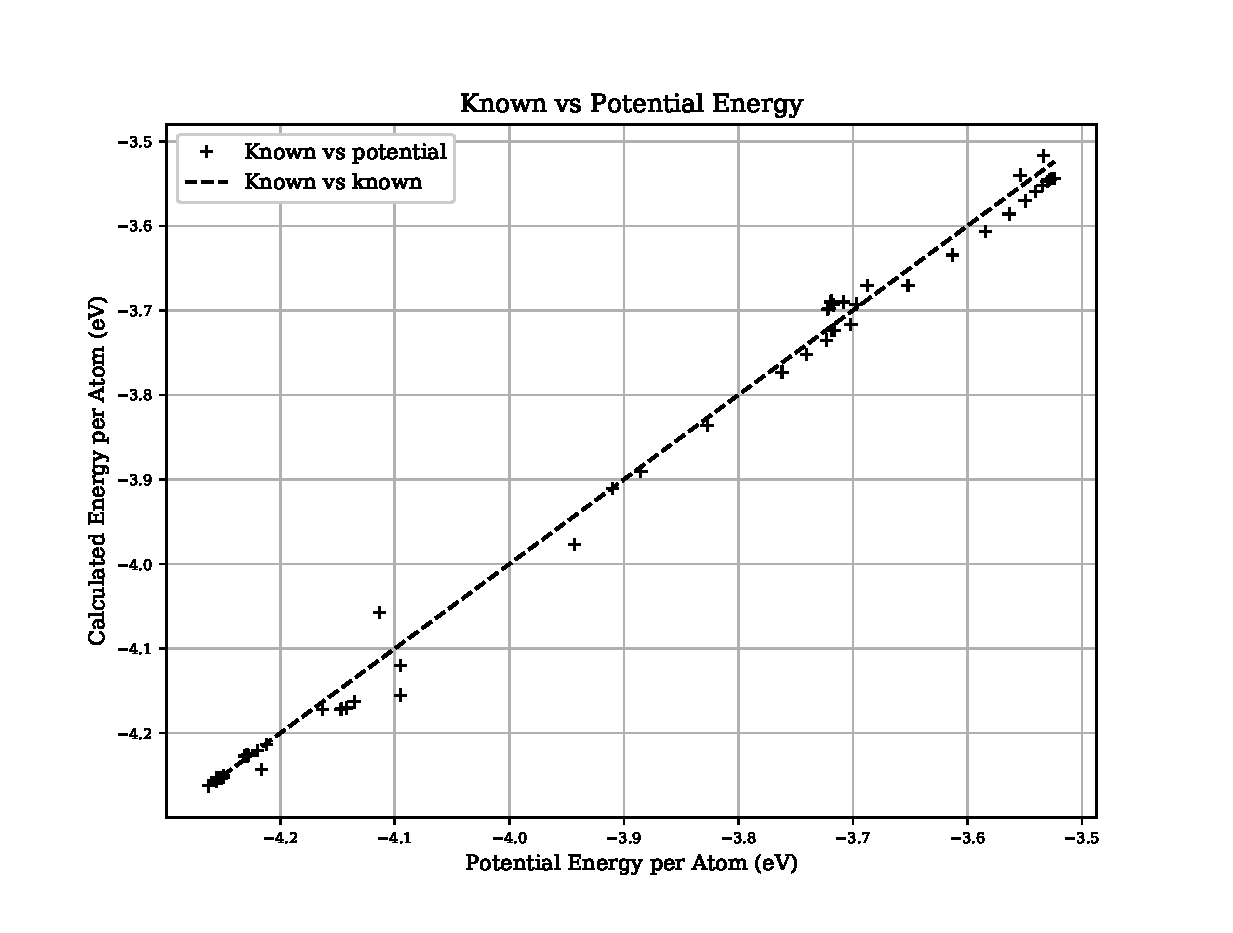
\includegraphics[width=.94\linewidth]{chapters/potentials_fe_pd_ru/fepd_potential/potential_known_energy_fit_set.eps}  
  \caption{DFT vs Potential, highly weighted configurations}
  \label{fig:fepd-energy-fit}
\end{subfigure}
\begin{subfigure}{.42\textwidth}
  \centering
  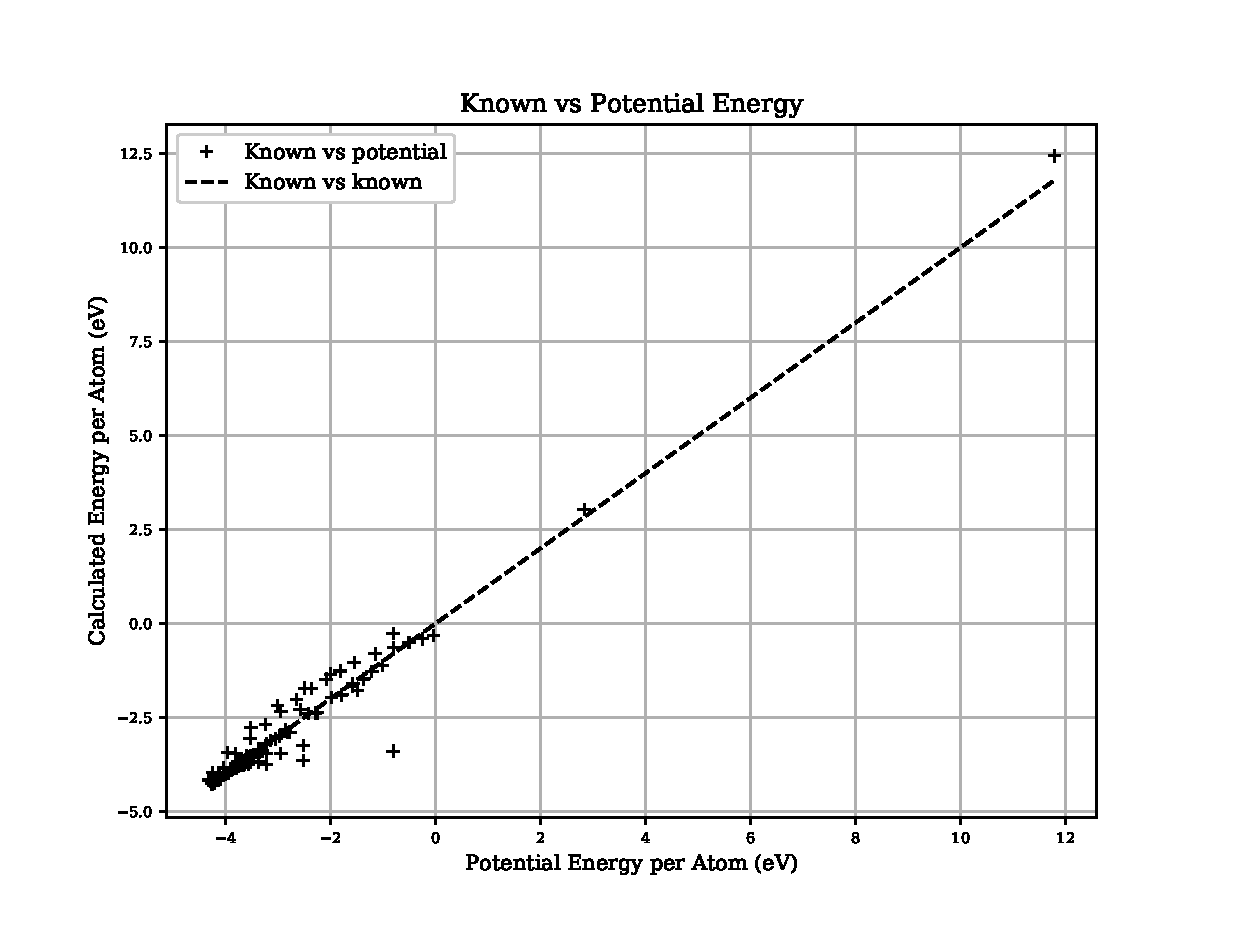
\includegraphics[width=.94\linewidth]{chapters/potentials_fe_pd_ru/fepd_potential/potential_known_energy_full_set.eps}  
  \caption{DFT vs Potential, all configurations}
  \label{fig:fepd-energy-full}
\end{subfigure}
\label{fig:fepd-energy}
\end{figure}

The \acrshort{dft} computed surface energy, as the slab forms from the increased gap between two surfaces, is given in figure \ref{fig:fepd-energy-fitting}.

\begin{figure}[htb]
\begin{subfigure}{.42\textwidth}
  \centering
  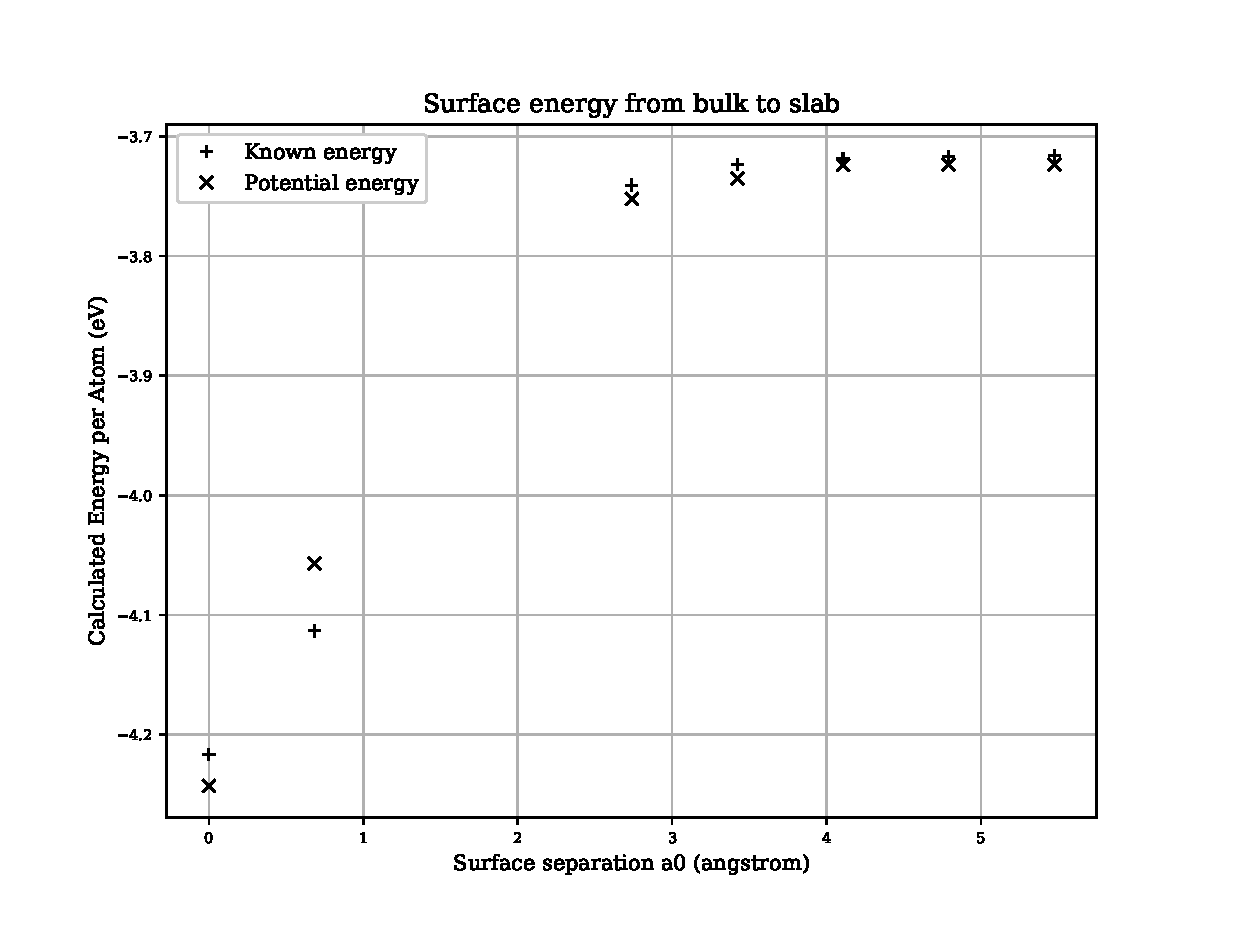
\includegraphics[width=.94\linewidth]{chapters/potentials_fe_pd_ru/fepd_potential/fe_surface_energy.eps}  
  \caption{Fe surface energy at a range of surface separations}
  \label{fig:fepd-fefcc-rose}
\end{subfigure}
\begin{subfigure}{.42\textwidth}
  \centering
  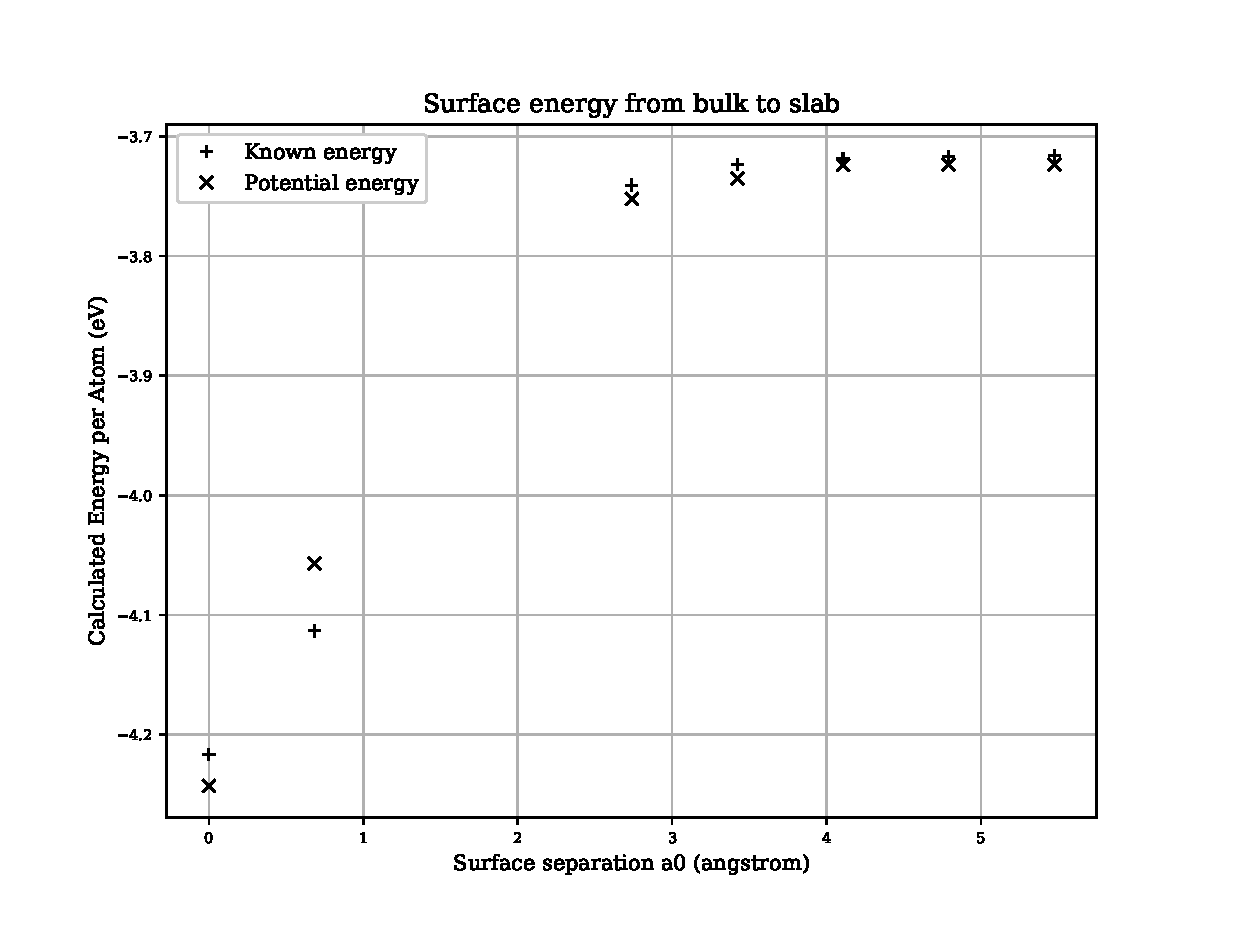
\includegraphics[width=.94\linewidth]{chapters/potentials_fe_pd_ru/fepd_potential/pd_surface_energy.eps}  
  \caption{Pd surface energy at a range of surface separations}
  \label{fig:fepd-fefcc-bmeos}
\end{subfigure}
\label{fig:fepd-energy-fitting}
\caption{Equation of State plots from this potential for \acrshort{fcc} Fe}
\end{figure}











\clearpage
\section{Bulk Properties}

%%%%%%%%%%%%%%%%%%%%%%%%%%%%%%%%%%%%%%%%%%%%%%%%%%%%%%%%%%%%%%%%%%%%%%
%  Iron FCC Bulk Properties
%%%%%%%%%%%%%%%%%%%%%%%%%%%%%%%%%%%%%%%%%%%%%%%%%%%%%%%%%%%%%%%%%%%%%%

\FloatBarrier
\subsection{Iron FCC}

\subsubsection{Bulk Property Values}

\begin{table}[ht]
\renewcommand{\arraystretch}{1.2}
\begin{tabular}{lcccccc}
\hline\hline
Property & \multicolumn{3}{c}{DFT Computed} & \multicolumn{3}{c}{This Potential} \\
\hline\hline
$a_0$ (angs)         & \multicolumn{3}{c}{3.42}   & \multicolumn{3}{c}{3.43} \\
Basis            & \multicolumn{3}{c}{$\begin{bmatrix} 1.0 & 0.0 & 0.0 \\ 0.0 & 1.05 & 0.0 \\ 0.0 & 0.0 & 1.0  \end{bmatrix}$} & \multicolumn{3}{c}{$\begin{bmatrix} 1.0 & 0.0 & 0.0 \\ 0.0 & 1.05 & 0.0 \\ 0.0 & 0.0 & 1.0  \end{bmatrix}$} \\
$E_{coh}$ (eV)           & \multicolumn{3}{c}{-4.26}  & \multicolumn{3}{c}{-4.27} \\
$B_0$ (GPa)              & \multicolumn{3}{c}{226.0}  & \multicolumn{3}{c}{297.2} \\
Stiff.1 (GPa) & \multicolumn{3}{c}{$\begin{bmatrix} 364.6 & 141.6 & 233.8 & 0 & 0 & 0 \\ 141.6 & 298.7 & 130.40 & 0 & 0 & 0 \\ 233.8 & 130.4 & 364.6 & 0 & 0 & 0 \\ 0 & 0 & 0 & 186.3 & 0 & 0 \\ 0 & 0 & 0 & 0 & 266.8 & 0 \\ 0 & 0 & 0 & 0 & 0 & 186.3 \end{bmatrix}$}   & \multicolumn{3}{c}{$\begin{bmatrix} 354.89 &  239.78 & 278.15 & 0 & 0 & 0 \\ 239.78 & 348.39 & 239.78 & 0 & 0 & 0 \\ 278.15 & 239.78 & 354.89 & 0 & 0 & 0 \\ 0 & 0 & 0 & 164.38 & 0 & 0 \\ 0 & 0 & 0 & 0 & 208.83 & 0 \\ 0 & 0 & 0 & 0 & 0 & 164.38 \end{bmatrix}$} \\
Stiff.2 (GPa) & \multicolumn{3}{c}{$\begin{bmatrix} 364.6 & 141.6 & 233.8 & 0 & 0 & 0 \\ 141.6 & 298.7 & 130.40 & 0 & 0 & 0 \\ 233.8 & 130.4 & 364.6 & 0 & 0 & 0 \\ 0 & 0 & 0 & 186.3 & 0 & 0 \\ 0 & 0 & 0 & 0 & 266.8 & 0 \\ 0 & 0 & 0 & 0 & 0 & 186.3 \end{bmatrix}$}   & \multicolumn{3}{c}{$\begin{bmatrix} 370.46 & 260.55 & 260.55 & 0 & 0 & 0 \\ 260.55 & 370.46 & 260.55 & 0 & 0 & 0 \\ 260.55 & 260.55 & 370.46 & 0 & 0 & 0 \\ 0 & 0 & 0 & 187.87 & 0 & 0 \\ 0 & 0 & 0 & 0 & 187.87 & 0 \\ 0 & 0 & 0 & 0 & 0 & 187.87 \end{bmatrix}$} \\
\hline\hline
\end{tabular}
\caption{The lattice parameter, cohesive energy and bulk modulus were determined by fitting the Birch-Murnaghan equation of state.  The elastic constants computed for the potential in stiffness (1) were computed using the method by Ravindran et al\cite{dfttisiravindran} and in stiffness (2) by Mehl et al\cite{mehlsp}\cite{elasticpropertiesmehl}.}
\label{table:fepd-fefcc-dftvspotential}
\end{table}


\subsubsection{Equation of State Plots}

Both the Birch-Murnaghan and Rose-Vinet equation of states are used in the fitting process.

\begin{figure}[htb]
\begin{subfigure}{.44\textwidth}
  \centering
  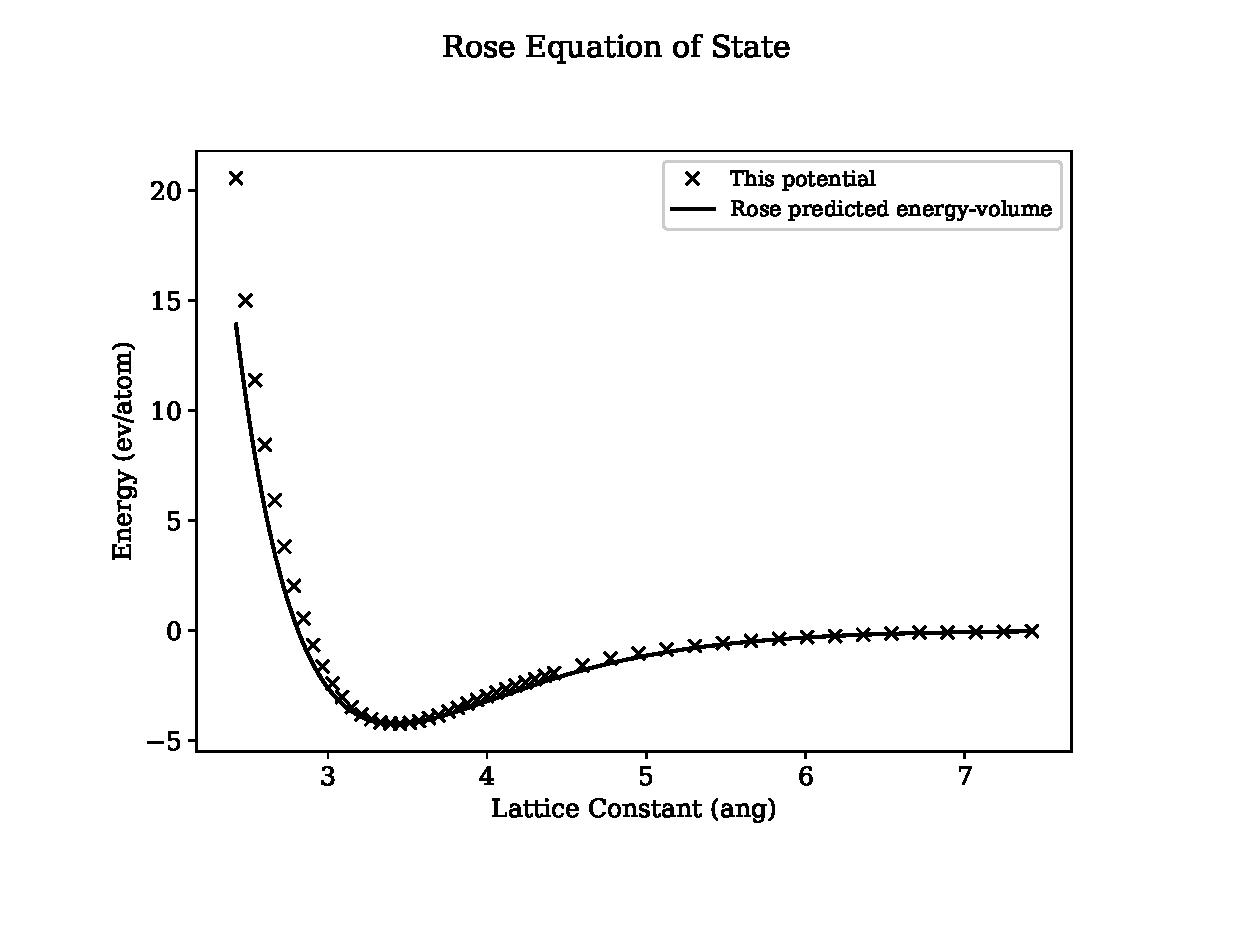
\includegraphics[width=.94\linewidth]{chapters/potentials_fe_pd_ru/fepd_potential/eos/rose_plot_bp_1.eps}  
  \caption{Rose-Vinet}
  \label{fig:fepd-fefcc-rose}
\end{subfigure}
\begin{subfigure}{.44\textwidth}
  \centering
  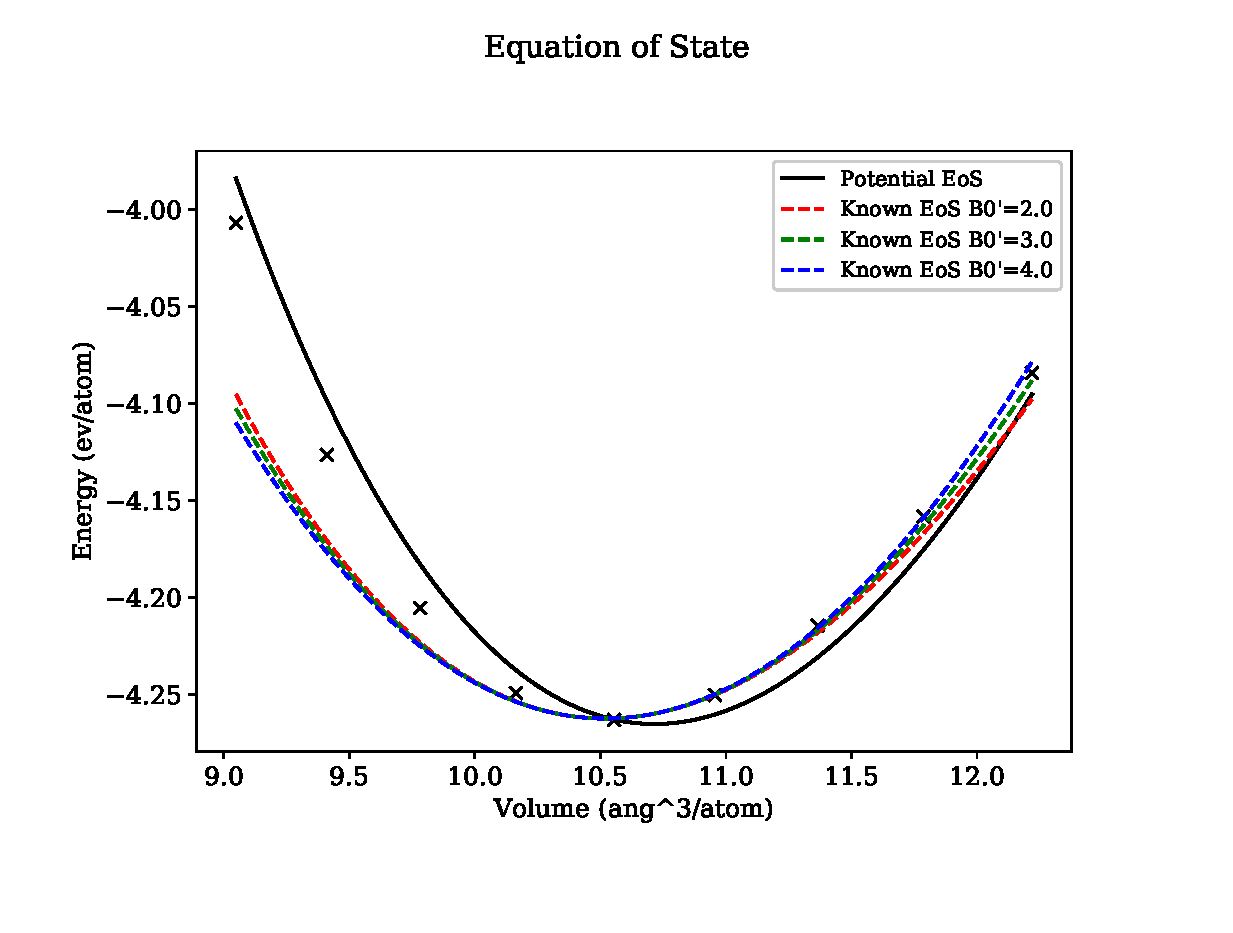
\includegraphics[width=.94\linewidth]{chapters/potentials_fe_pd_ru/fepd_potential/eos/equation_of_state_bp_1.eps}  
  \caption{Birch Murnaghan}
  \label{fig:fepd-fefcc-bmeos}
\end{subfigure}
\label{fig:fepd-fefcc-equation-of-state}
\caption{Equation of State plots from this potential for \acrshort{fcc} Fe}
\end{figure}


\clearpage
\subsubsection{Elastic Constant Plots}

\begin{figure}[htb]
\centering
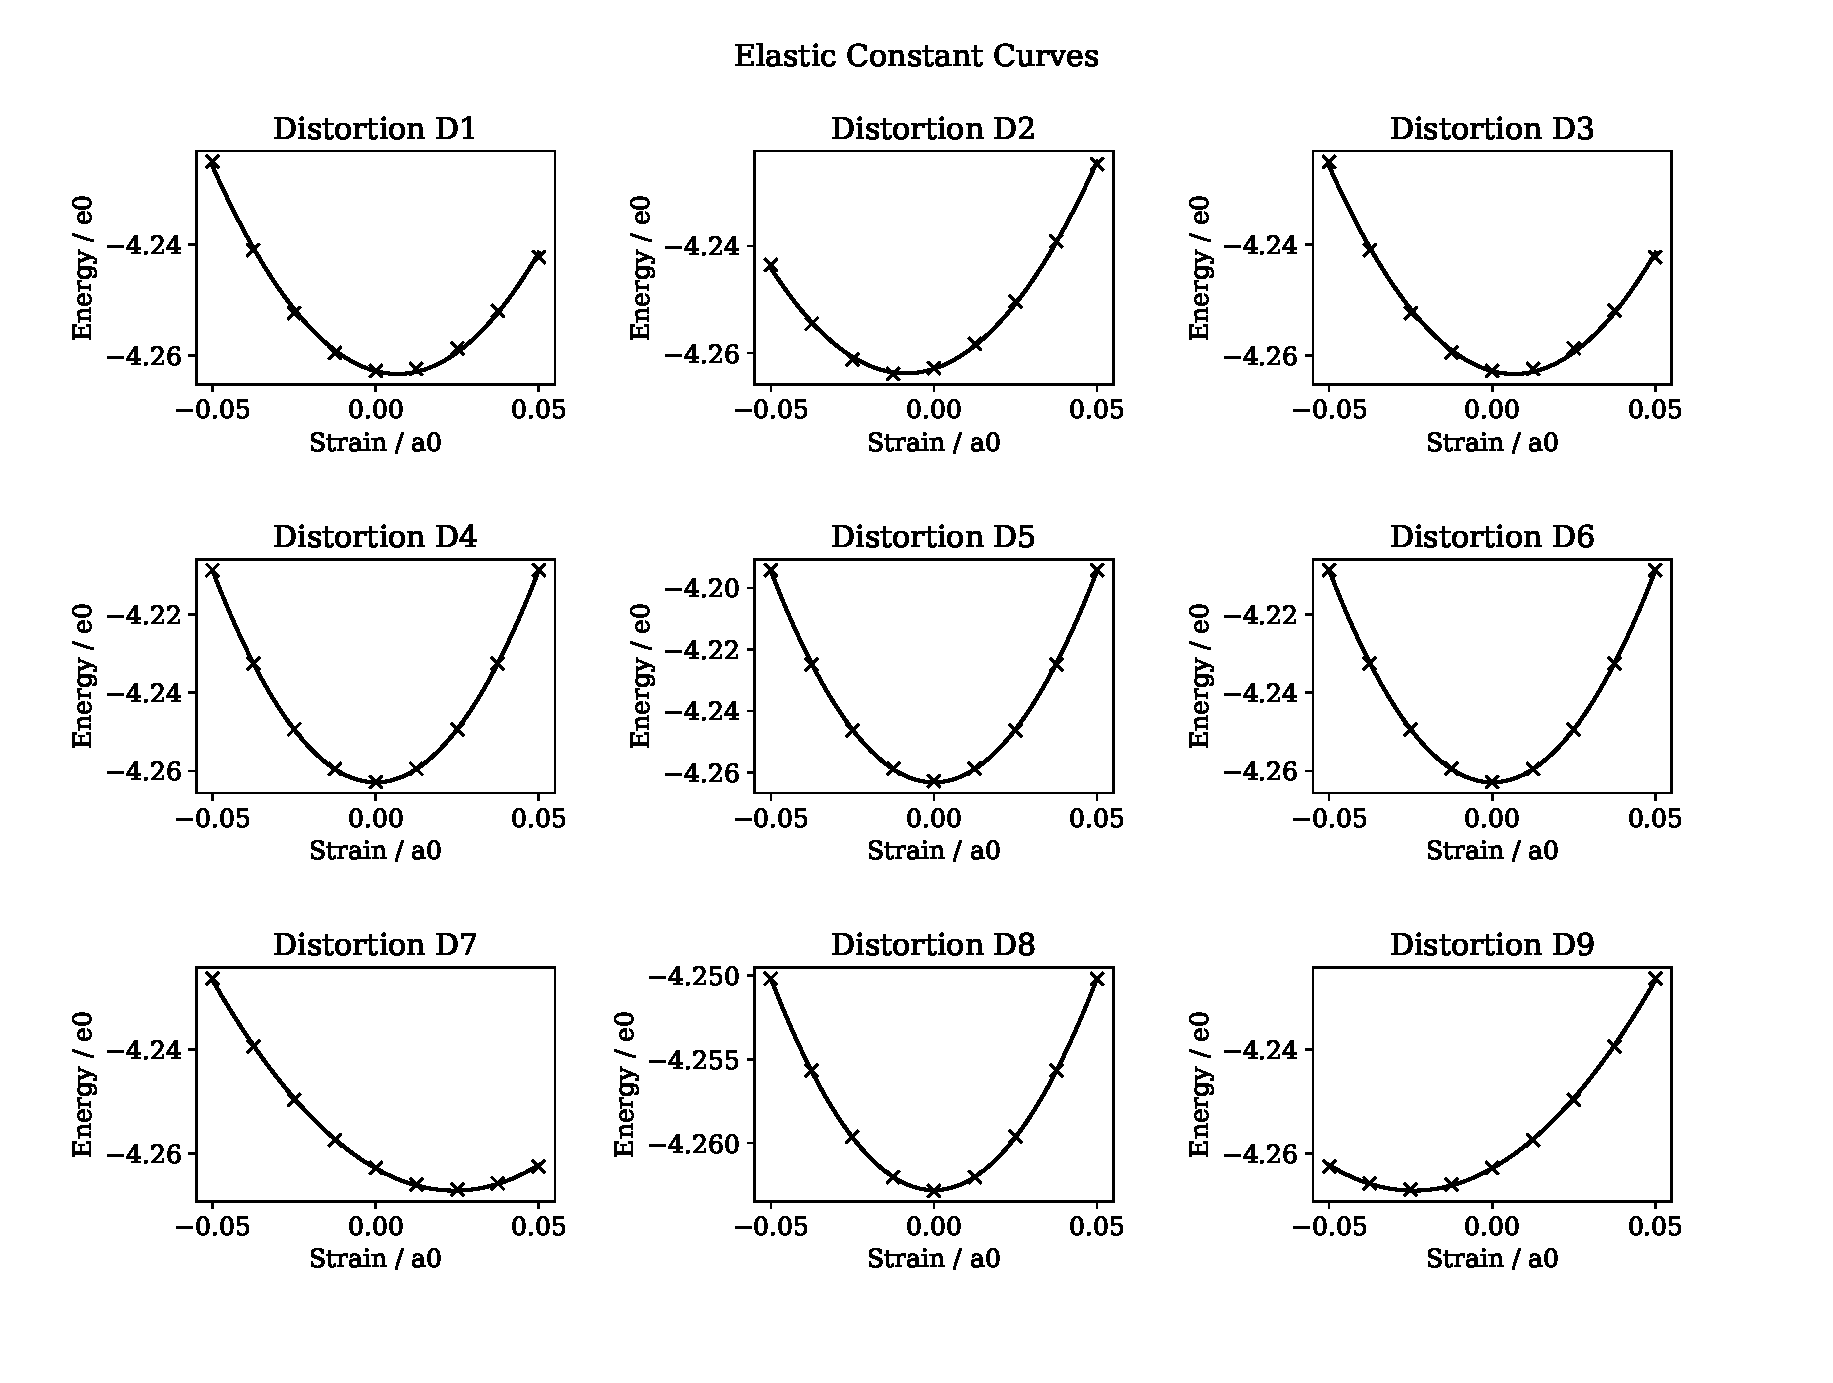
\includegraphics[width=.90\linewidth]{chapters/potentials_fe_pd_ru/fepd_potential/ec_rfkj/elastic_strains_bp_1.eps}  
\label{fig:fepd-fefcc-distortions}
\caption{Ravindran et al\cite{dfttisiravindran} distortion-energy plots for \acrshort{fcc} Fe}
\end{figure}

\begin{figure}[htb]
\begin{subfigure}{.42\textwidth}
  \centering
  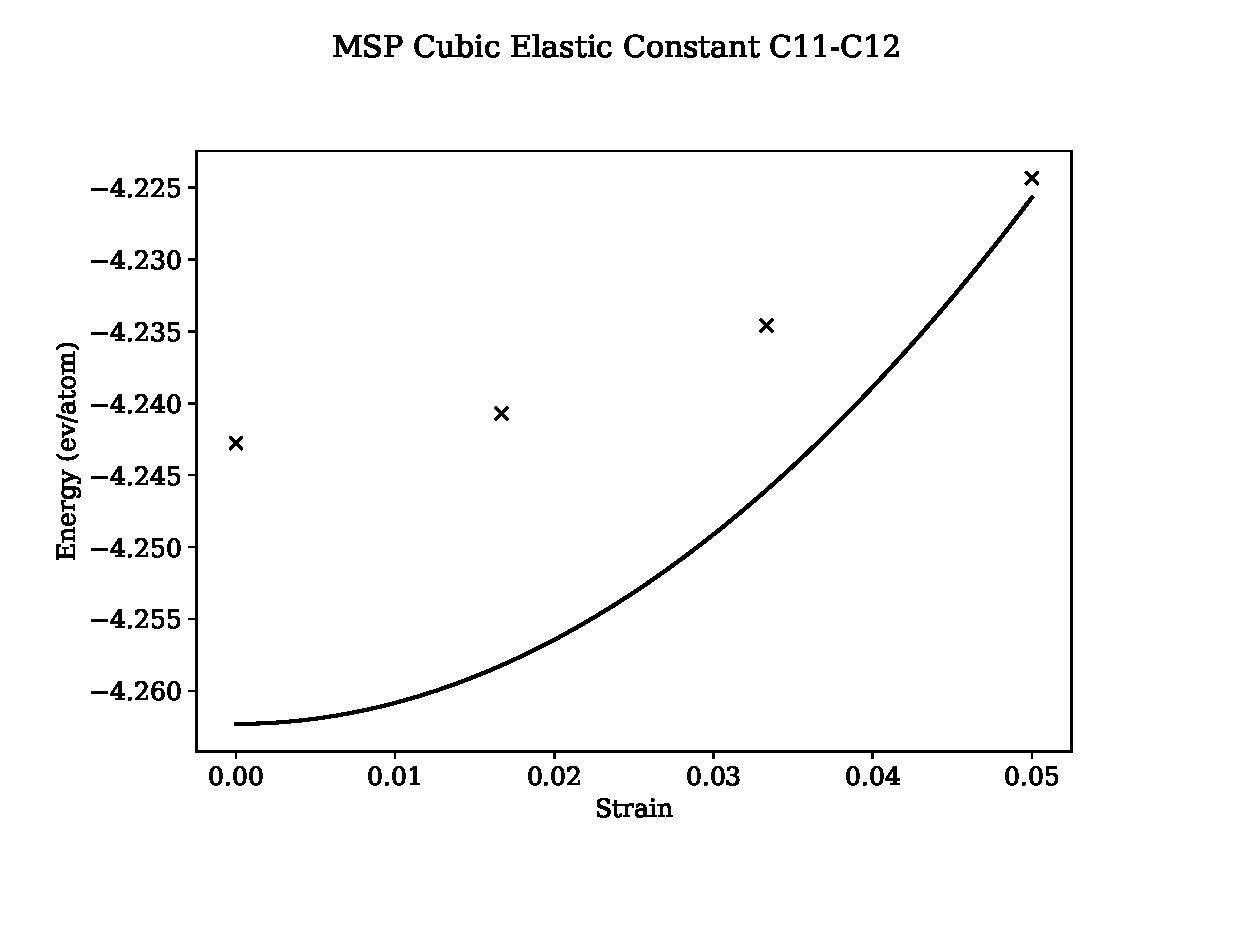
\includegraphics[width=.90\linewidth]{chapters/potentials_fe_pd_ru/fepd_potential/ec_mskp/msp_c11_c12_plot_bp_1.eps}  
  \caption{C11-C12 orthorhombic distortion}
  \label{fig:fepd-fefcc-c11c12}
\end{subfigure}
\begin{subfigure}{.42\textwidth}
  \centering
  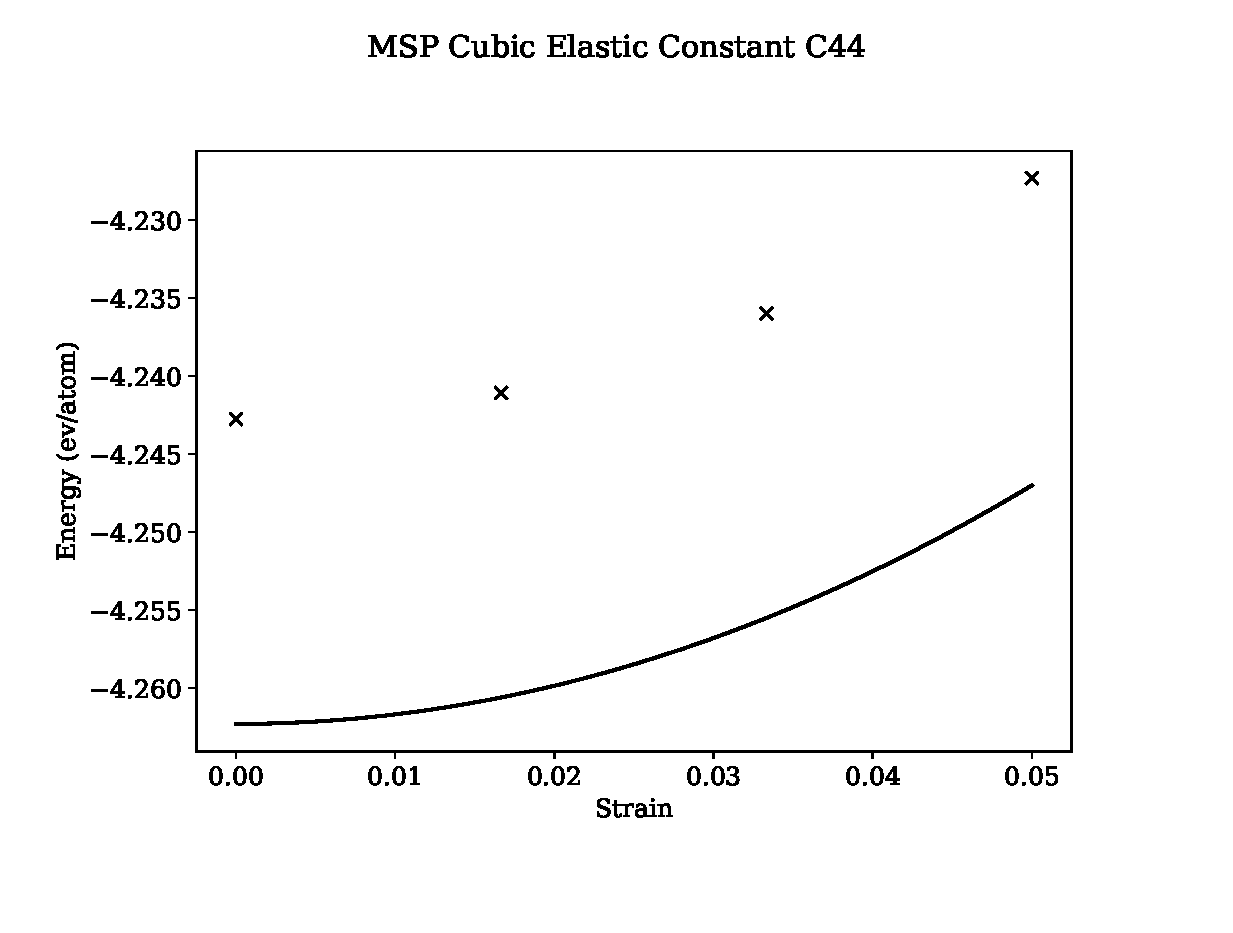
\includegraphics[width=.90\linewidth]{chapters/potentials_fe_pd_ru/fepd_potential/ec_mskp/msp_c44_plot_bp_1.eps}  
  \caption{C44 monoclinic distortion}
  \label{fig:fepd-fefcc-c11c12c44}
\end{subfigure}
\label{fig:fig:fepd-fefcc-equation-of-state}
\caption{Equation of State plots from this potential for \acrshort{fcc} Fe}
\end{figure}







%%%%%%%%%%%%%%%%%%%%%%%%%%%%%%%%%%%%%%%%%%%%%%%%%%%%%%%%%%%%%%%%%%%%%%
%  Palladium FCC Bulk Properties
%%%%%%%%%%%%%%%%%%%%%%%%%%%%%%%%%%%%%%%%%%%%%%%%%%%%%%%%%%%%%%%%%%%%%%

\clearpage
\FloatBarrier
\subsection{Palladium FCC}

\begin{table}[ht]
\renewcommand{\arraystretch}{1.2}
\begin{tabular}{lcccccc}
\hline\hline
Property & \multicolumn{3}{c}{DFT Computed} & \multicolumn{3}{c}{This Potential} \\
\hline\hline
$a_0$ (angs)         & \multicolumn{3}{c}{3.93}   & \multicolumn{3}{c}{3.94} \\
Basis            & \multicolumn{3}{c}{$\begin{bmatrix} 1.0 & 0.0 & 0.0 \\ 0.0 & 1.0 & 0.0 \\ 0.0 & 0.0 & 1.0  \end{bmatrix}$} & \multicolumn{3}{c}{$\begin{bmatrix} 1.0 & 0.0 & 0.0 \\ 0.0 & 1.0 & 0.0 \\ 0.0 & 0.0 & 1.0  \end{bmatrix}$} \\
$E_{coh}$ (eV)           & \multicolumn{3}{c}{-4.316}  & \multicolumn{3}{c}{-4.159} \\
$B_0$ (GPa)              & \multicolumn{3}{c}{170.0}  & \multicolumn{3}{c}{253.0} \\
Stiff.1 (GPa) & \multicolumn{3}{c}{$\begin{bmatrix} 243.0 & 145.0 & 145.0 & 0 & 0 & 0 \\ 145.0 & 243.0 & 145.0 & 0 & 0 & 0 \\ 145.0 & 145.0 & 243.0 & 0 & 0 & 0 \\ 0 & 0 & 0 & 116.0 & 0 & 0 \\ 0 & 0 & 0 & 0 & 116.0 & 0 \\ 0 & 0 & 0 & 0 & 0 & 116.0 \end{bmatrix}$}   & \multicolumn{3}{c}{$\begin{bmatrix} 214.54 & 242.49 & 242.49 & 0 & 0 & 0 \\ 242.49 & 214.54 & 242.49 & 0 & 0 & 0 \\ 242.49 & 242.49 & 214.54 & 0 & 0 & 0 \\ 0 & 0 & 0 & 178.94 & 0 & 0 \\ 0 & 0 & 0 & 0 & 178.94 & 0 \\ 0 & 0 & 0 & 0 & 0 & 178.94 \end{bmatrix}$} \\
Stiff.2 (GPa) & \multicolumn{3}{c}{$\begin{bmatrix} 243.0 & 145.0 & 145.0 & 0 & 0 & 0 \\ 145.0 & 243.0 & 145.0 & 0 & 0 & 0 \\ 145.0 & 145.0 & 243.0 & 0 & 0 & 0 \\ 0 & 0 & 0 & 116.0 & 0 & 0 \\ 0 & 0 & 0 & 0 & 116.0 & 0 \\ 0 & 0 & 0 & 0 & 0 & 116.0 \end{bmatrix}$}   & \multicolumn{3}{c}{$\begin{bmatrix} 240.70 & 259.10 & 259.10 & 0 & 0 & 0 \\ 259.10 & 240.70 & 259.10 & 0 & 0 & 0 \\ 259.10 & 259.10 & 240.70 & 0 & 0 & 0 \\ 0 & 0 & 0 & 164.19 & 0 & 0 \\ 0 & 0 & 0 & 0 & 164.19 & 0 \\ 0 & 0 & 0 & 0 & 0 & 164.19 \end{bmatrix}$} \\
\hline\hline
\end{tabular}
\caption{The lattice parameter, cohesive energy and bulk modulus were determined by fitting the Birch-Murnaghan equation of state.  The elastic constants computed for the potential in stiffness (1) were computed using the method by Ravindran et al\cite{dfttisiravindran} and in stiffness (2) by Mehl et al\cite{mehlsp}\cite{elasticpropertiesmehl}.}
\label{table:fepd-pdfcc-dftvspotential}
\end{table}



\subsubsection{Equation of State Plots}

Both the Birch-Murnaghan and Rose-Vinet equation of states are used in the fitting process.

\begin{figure}[htb]
\begin{subfigure}{.44\textwidth}
  \centering
  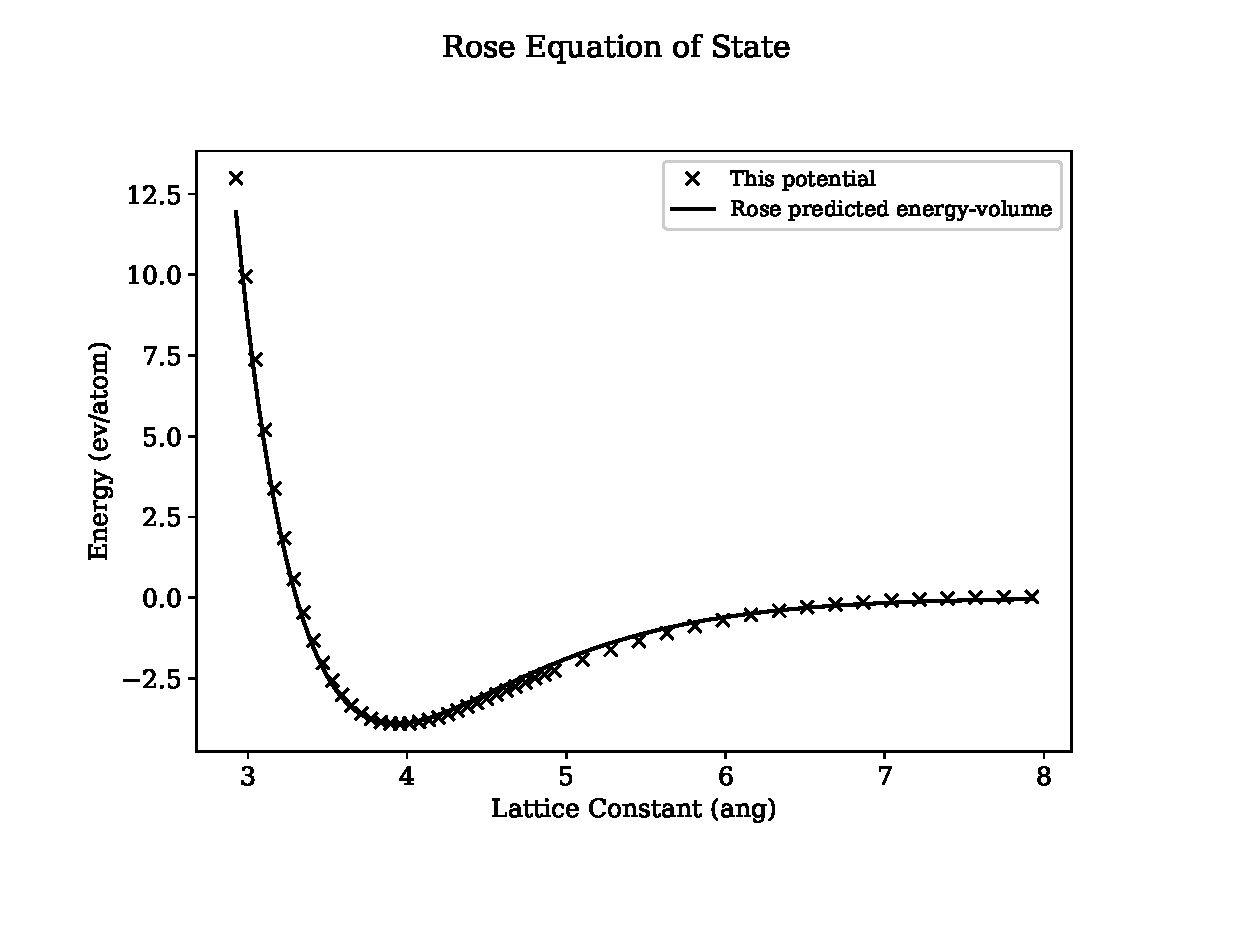
\includegraphics[width=.94\linewidth]{chapters/potentials_fe_pd_ru/fepd_potential/eos/rose_plot_bp_2.eps}  
  \caption{Rose-Vinet}
  \label{fig:fepd-fefcc-rose}
\end{subfigure}
\begin{subfigure}{.44\textwidth}
  \centering
  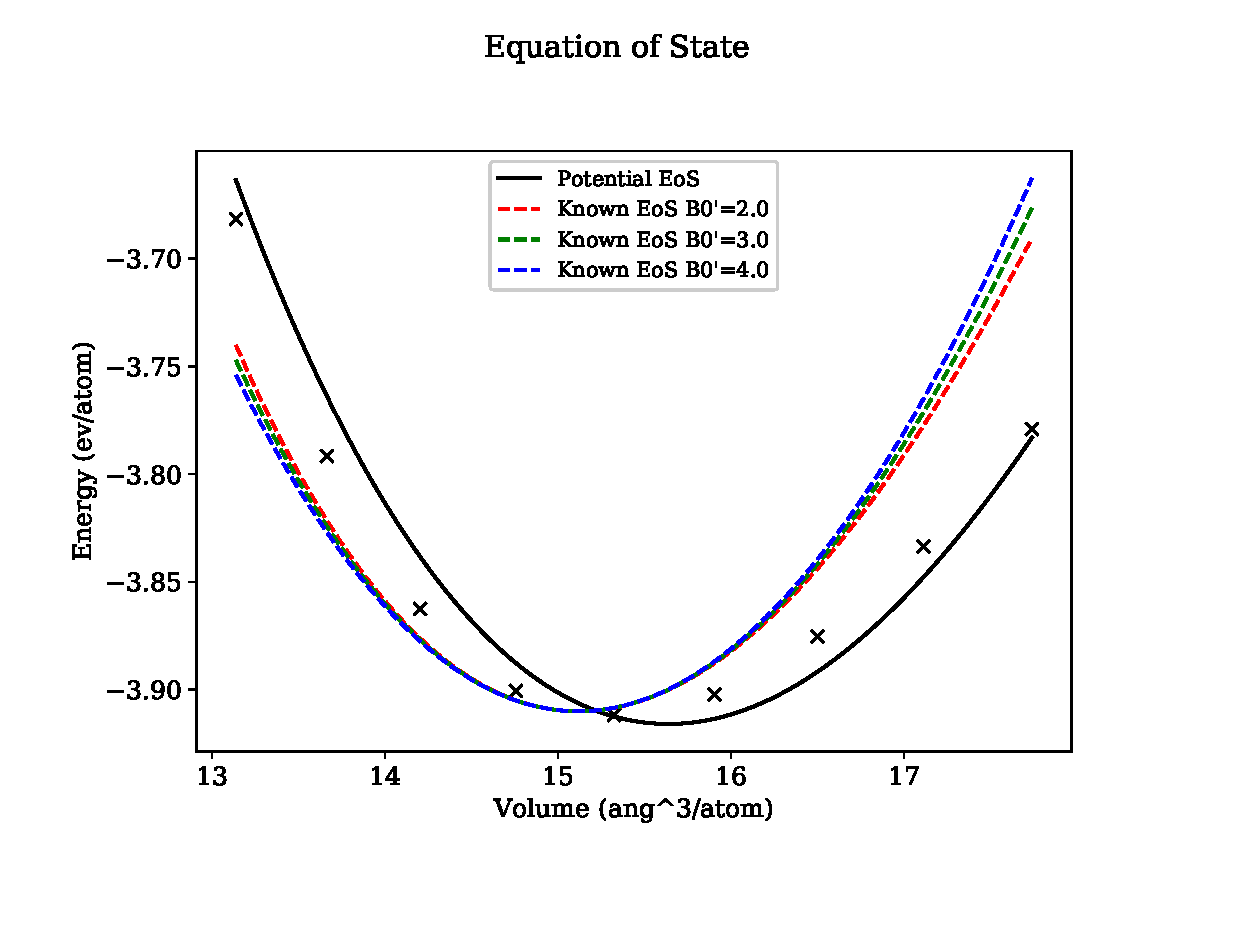
\includegraphics[width=.94\linewidth]{chapters/potentials_fe_pd_ru/fepd_potential/eos/equation_of_state_bp_2.eps}  
  \caption{Birch Murnaghan}
  \label{fig:fepd-fefcc-bmeos}
\end{subfigure}
\label{fig:fepd-fefcc-equation-of-state}
\caption{Equation of State plots from this potential for \acrshort{fcc} Pd}
\end{figure}


\clearpage
\subsubsection{Elastic Constant Plots}

\begin{figure}[htb]
\centering
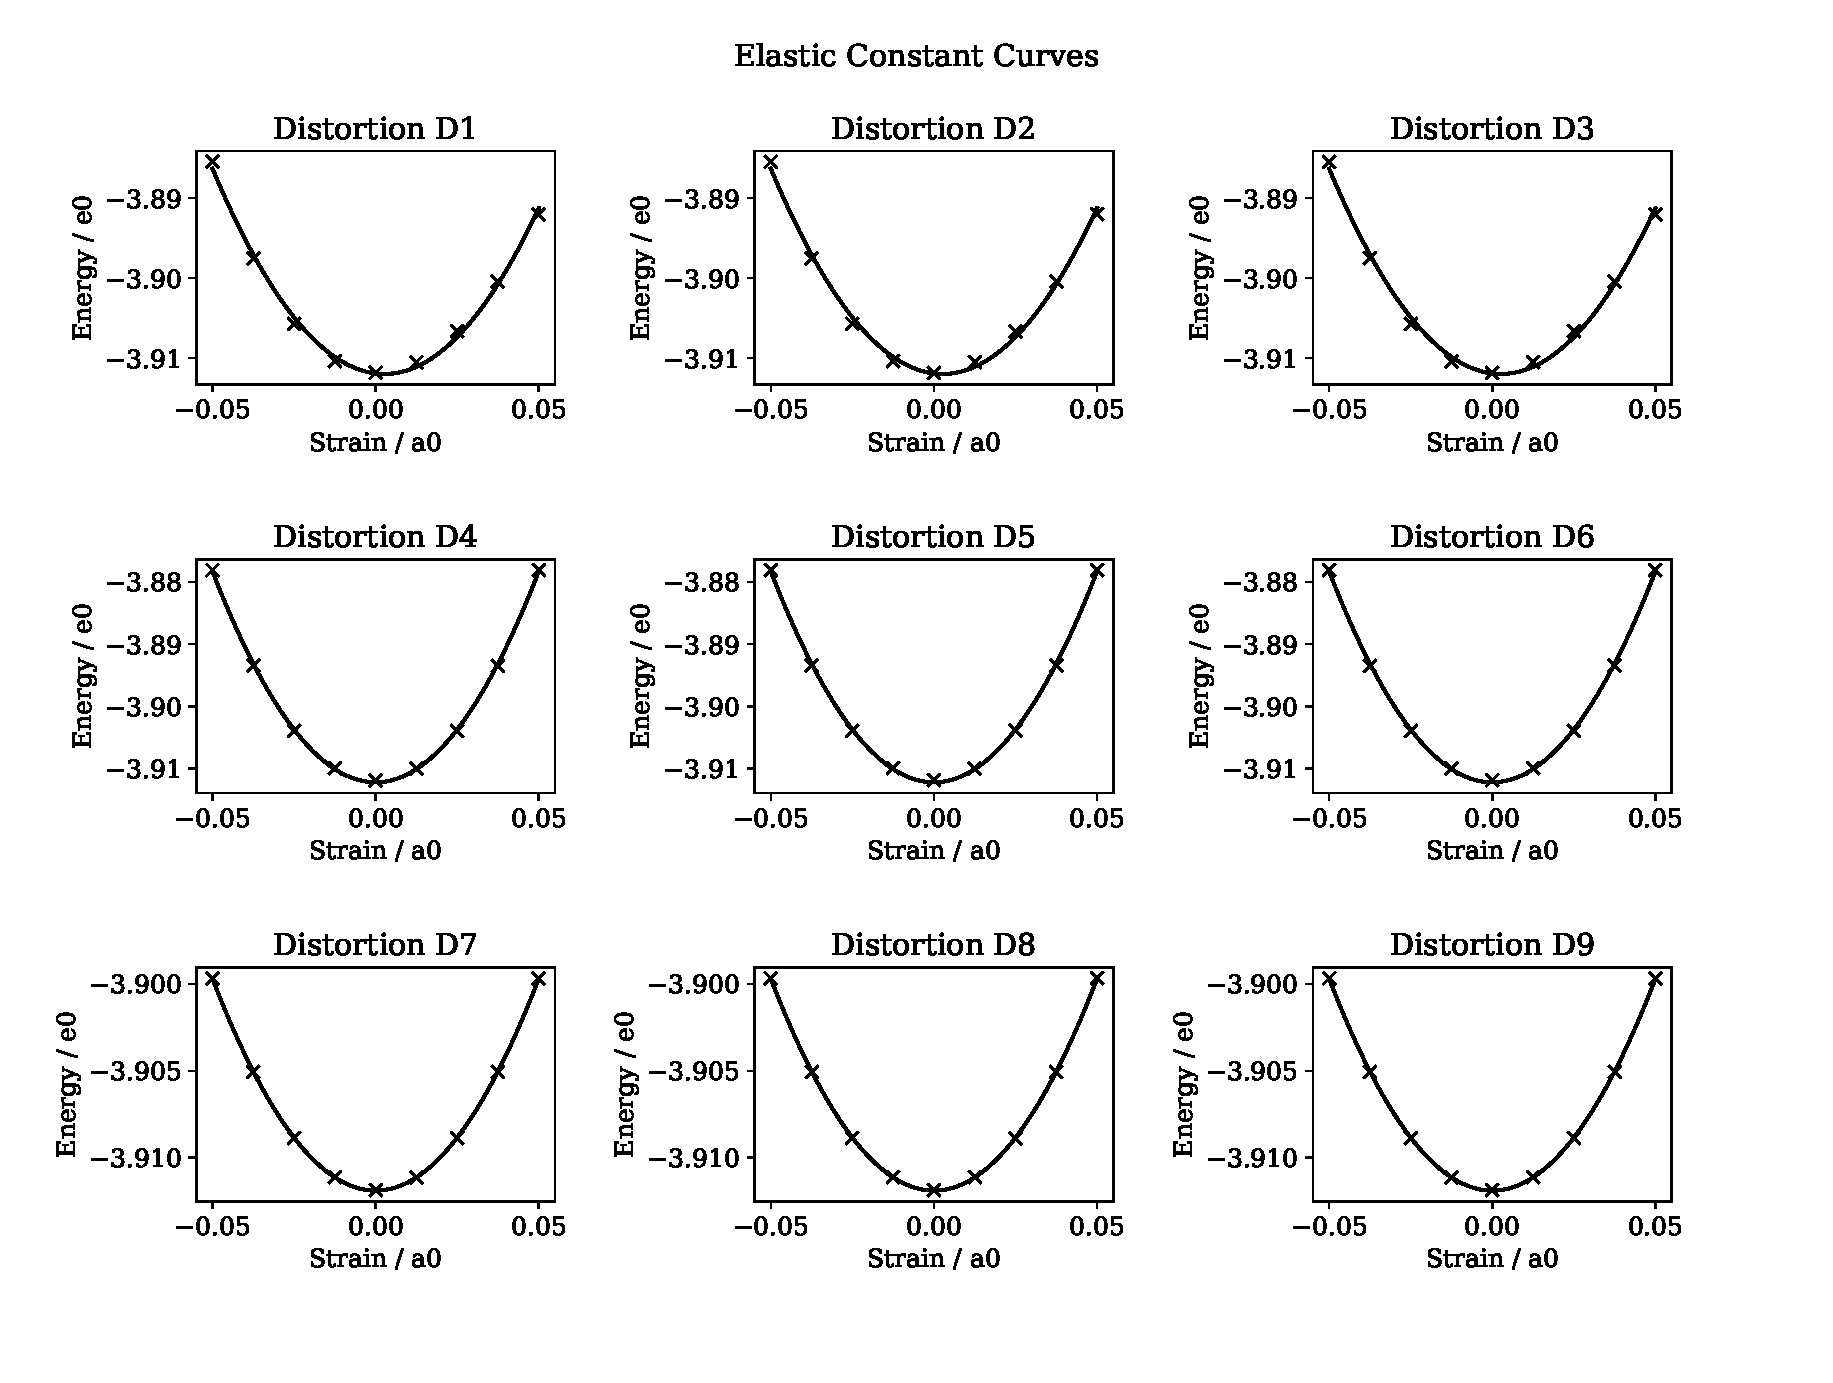
\includegraphics[width=.90\linewidth]{chapters/potentials_fe_pd_ru/fepd_potential/ec_rfkj/elastic_strains_bp_2.eps}  
\label{fig:fepd-pdfcc-distortions}
\caption{Ravindran et al\cite{dfttisiravindran} distortion-energy plots for \acrshort{fcc} Pd}
\end{figure}

\begin{figure}[htb]
\begin{subfigure}{.42\textwidth}
  \centering
  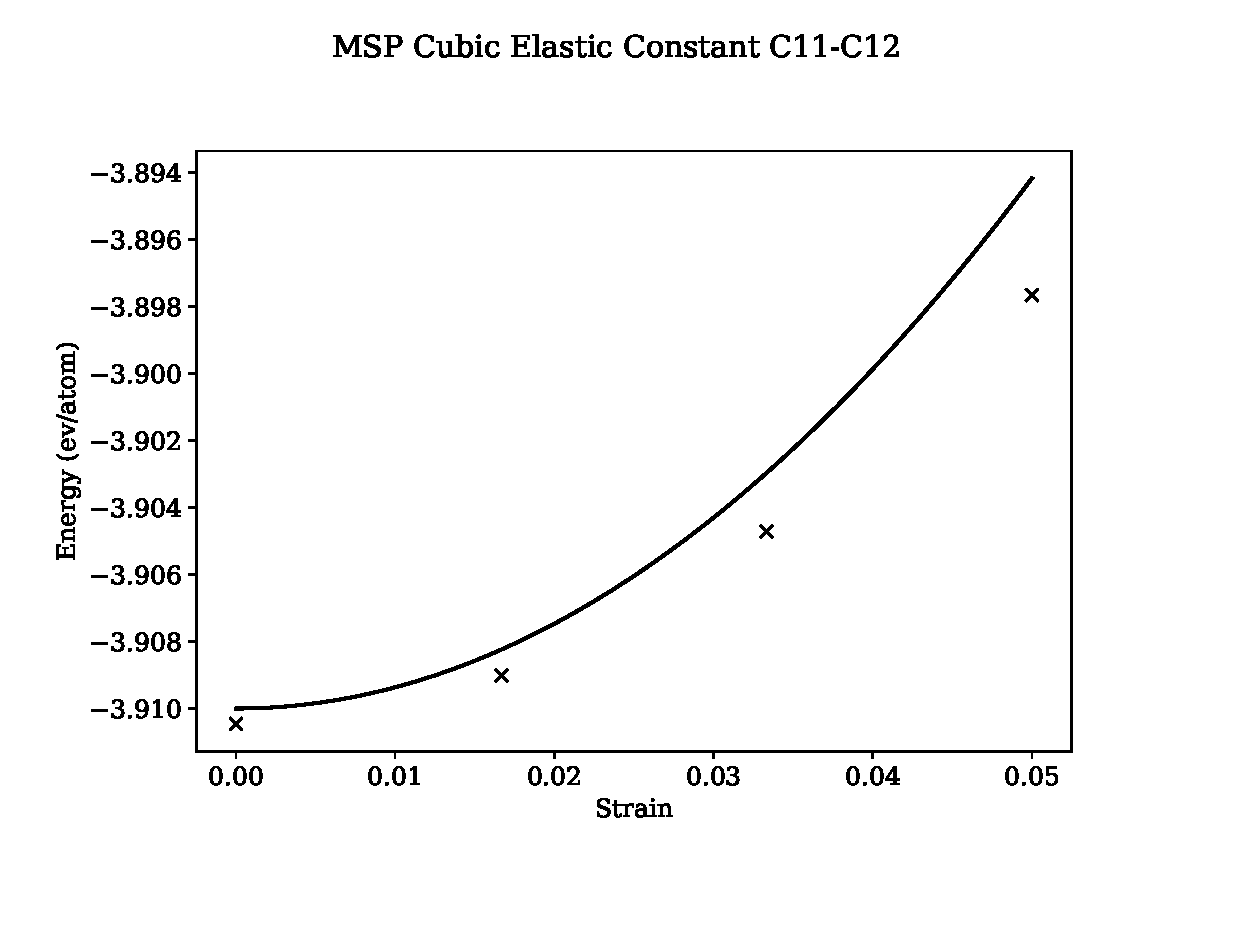
\includegraphics[width=.90\linewidth]{chapters/potentials_fe_pd_ru/fepd_potential/ec_mskp/msp_c11_c12_plot_bp_2.eps}  
  \caption{C11-C12 orthorhombic distortion}
  \label{fig:fepd-pdfcc-c11c12}
\end{subfigure}
\begin{subfigure}{.42\textwidth}
  \centering
  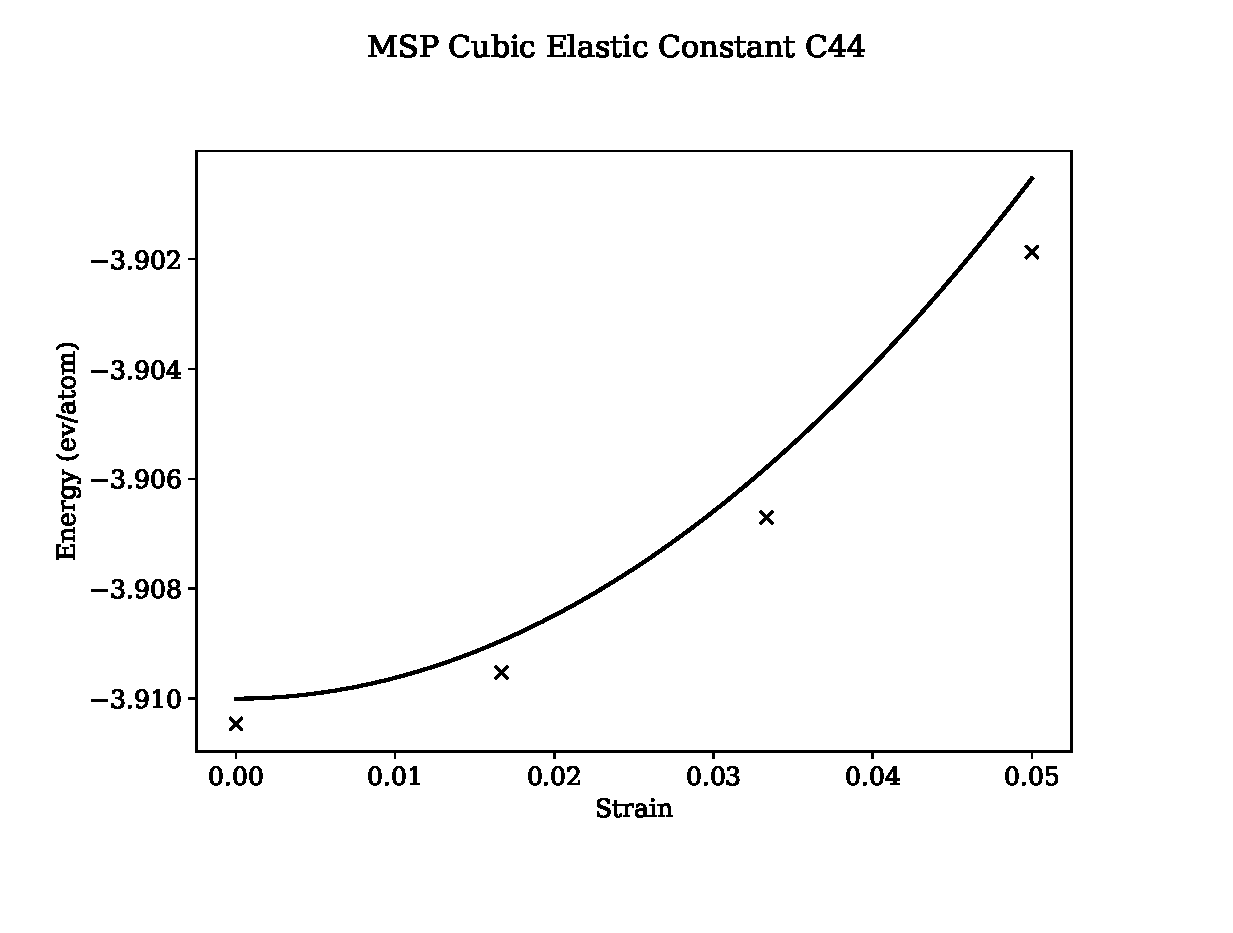
\includegraphics[width=.90\linewidth]{chapters/potentials_fe_pd_ru/fepd_potential/ec_mskp/msp_c44_plot_bp_2.eps}  
  \caption{C44 monoclinic distortion}
  \label{fig:fepd-pdfcc-c44}
\end{subfigure}
\label{fig:fepd-fefcc-c11c12c44}
\caption{Equation of State plots from this potential for \acrshort{fcc} Pd}
\end{figure}



%%%%%%%%%%%%%%%%%%%%%%%%%%%%%%%%%%%%%%%%%%%%%%%%%%%%%%%%%%%%%%%%%%%%%%
%  Iron BCC Bulk Properties
%%%%%%%%%%%%%%%%%%%%%%%%%%%%%%%%%%%%%%%%%%%%%%%%%%%%%%%%%%%%%%%%%%%%%%

\clearpage
\FloatBarrier
\subsection{Iron BCC}


\begin{table}[ht]
\renewcommand{\arraystretch}{1.2}
\begin{tabular}{lcccccc}
\hline\hline
Property & \multicolumn{3}{c}{DFT Computed} & \multicolumn{3}{c}{This Potential} \\
\hline\hline
$a_0$ (angs)         & \multicolumn{3}{c}{2.86}   & \multicolumn{3}{c}{2.77} \\
Basis            & \multicolumn{3}{c}{$\begin{bmatrix} 1.0 & 0.0 & 0.0 \\ 0.0 & 1.0 & 0.0 \\ 0.0 & 0.0 & 1.0  \end{bmatrix}$} & \multicolumn{3}{c}{$\begin{bmatrix} 1.0 & 0.0 & 0.0 \\ 0.0 & 1.0 & 0.0 \\ 0.0 & 0.0 & 1.0  \end{bmatrix}$} \\
$E_{coh}$ (eV)           & \multicolumn{3}{c}{-3.91}  & \multicolumn{3}{c}{--3.92} \\
$B_0$ (GPa)              & \multicolumn{3}{c}{184.0}  & \multicolumn{3}{c}{172.3} \\
Stiff.1 (GPa) & \multicolumn{3}{c}{$\begin{bmatrix} 218.5 & 151.4 & 151.4 & 0 & 0 & 0 \\ 151.4 & 218.5 & 151.4 & 0 & 0 & 0 \\ 151.4 & 151.4 & 218.5 & 0 & 0 & 0 \\ 0 & 0 & 0 & 80.3 & 0 & 0 \\ 0 & 0 & 0 & 0 & 80.3 & 0 \\ 0 & 0 & 0 & 0 & 0 & 80.3 \end{bmatrix}$}   & \multicolumn{3}{c}{$\begin{bmatrix} 193.52 & 142.54 & 142.54 & 0 & 0 & 0 \\ 142.54 & 193.52 & 142.54 & 0 & 0 & 0 \\ 142.54 & 142.54 & 193.52 & 0 & 0 & 0 \\ 0 & 0 & 0 & 70.86 & 0 & 0 \\ 0 & 0 & 0 & 0 & 70.86 & 0 \\ 0 & 0 & 0 & 0 & 0 & 70.86 \end{bmatrix}$} \\
Stiff.2 (GPa) & \multicolumn{3}{c}{$\begin{bmatrix} 218.5 & 151.4 & 151.4 & 0 & 0 & 0 \\ 151.4 & 218.5 & 151.4 & 0 & 0 & 0 \\ 151.4 & 151.4 & 218.5 & 0 & 0 & 0 \\ 0 & 0 & 0 & 80.3 & 0 & 0 \\ 0 & 0 & 0 & 0 & 80.3 & 0 \\ 0 & 0 & 0 & 0 & 0 & 80.3 \end{bmatrix}$}   & \multicolumn{3}{c}{$\begin{bmatrix} 206.76 & 155.09 & 155.09 & 0 & 0 & 0 \\ 155.09 & 206.76 & 155.09 & 0 & 0 & 0 \\ 155.09 & 155.09 & 206.76 & 0 & 0 & 0 \\ 0 & 0 & 0 & 71.77 & 0 & 0 \\ 0 & 0 & 0 & 0 & 71.77 & 0 \\ 0 & 0 & 0 & 0 & 0 & 71.77 \end{bmatrix}$} \\
\hline\hline
\end{tabular}
\caption{The lattice parameter, cohesive energy and bulk modulus were determined by fitting the Birch-Murnaghan equation of state.  The elastic constants computed for the potential in stiffness (1) were computed using the method by Ravindran et al\cite{dfttisiravindran} and in stiffness (2) by Mehl et al\cite{mehlsp}\cite{elasticpropertiesmehl}.}
\label{table:fepd-febcc-dftvspotential}
\end{table}



\subsubsection{Equation of State Plots}

Both the Birch-Murnaghan and Rose-Vinet equation of states are used in the fitting process.

\begin{figure}[htb]
\begin{subfigure}{.44\textwidth}
  \centering
  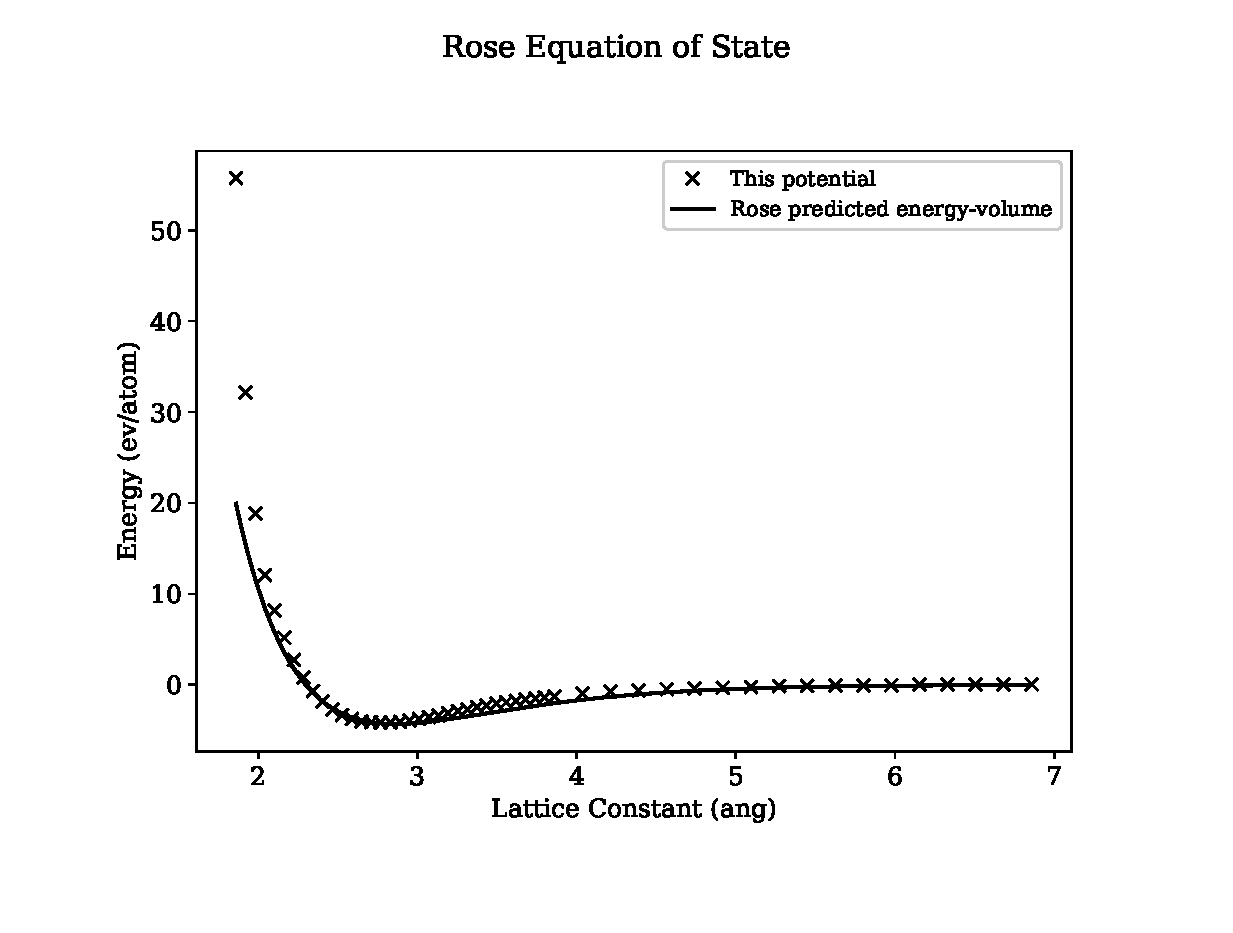
\includegraphics[width=.94\linewidth]{chapters/potentials_fe_pd_ru/fepd_potential/eos/rose_plot_bp_0.eps}  
  \caption{Rose-Vinet}
  \label{fig:fepd-fefcc-rose}
\end{subfigure}
\begin{subfigure}{.44\textwidth}
  \centering
  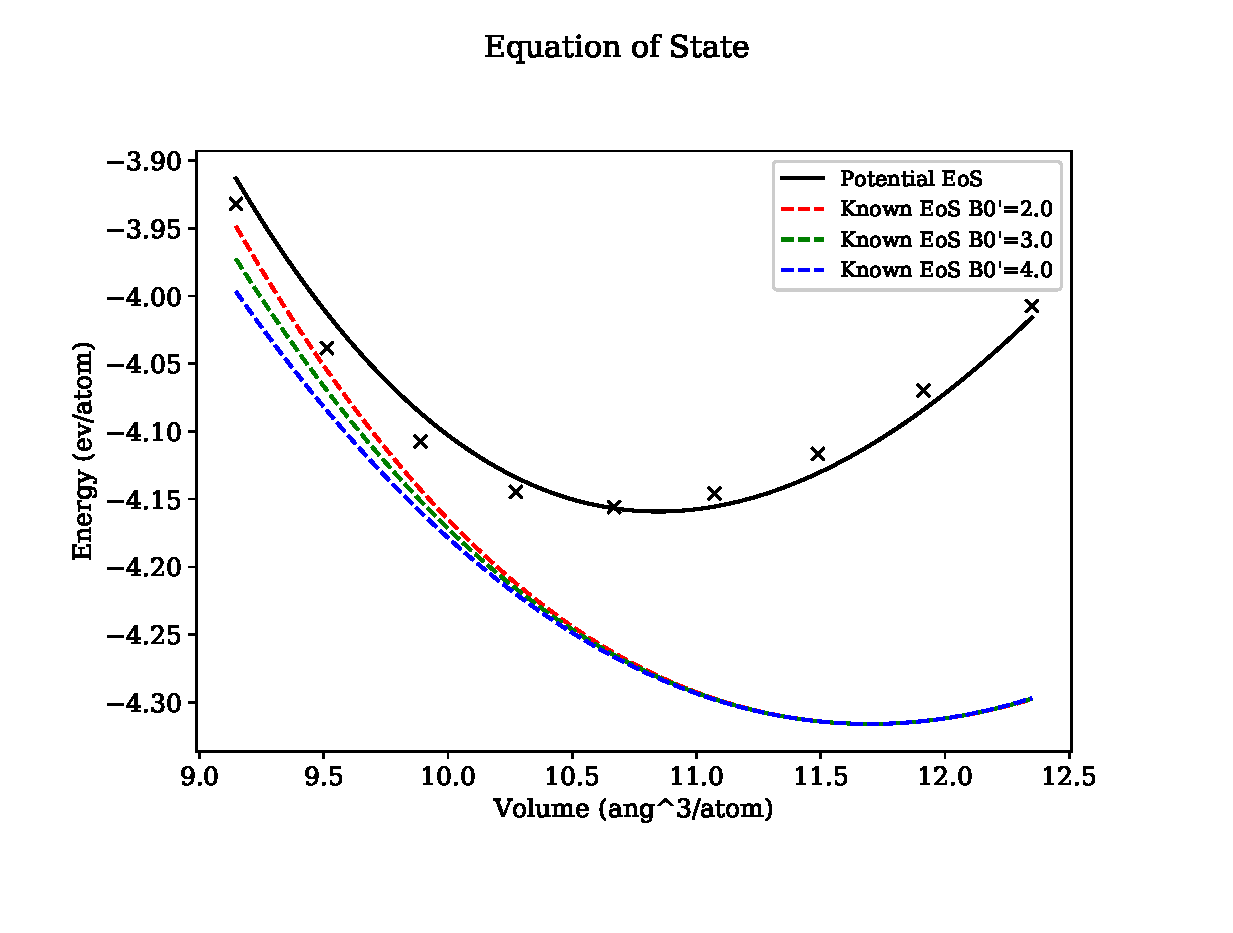
\includegraphics[width=.94\linewidth]{chapters/potentials_fe_pd_ru/fepd_potential/eos/equation_of_state_bp_0.eps}  
  \caption{Birch Murnaghan}
  \label{fig:fepd-fefcc-bmeos}
\end{subfigure}
\label{fig:fepd-fefcc-equation-of-state}
\caption{Equation of State plots from this potential for \acrshort{fcc} Pd}
\end{figure}


\clearpage
\subsubsection{Elastic Constant Plots}

\begin{figure}[htb]
\centering
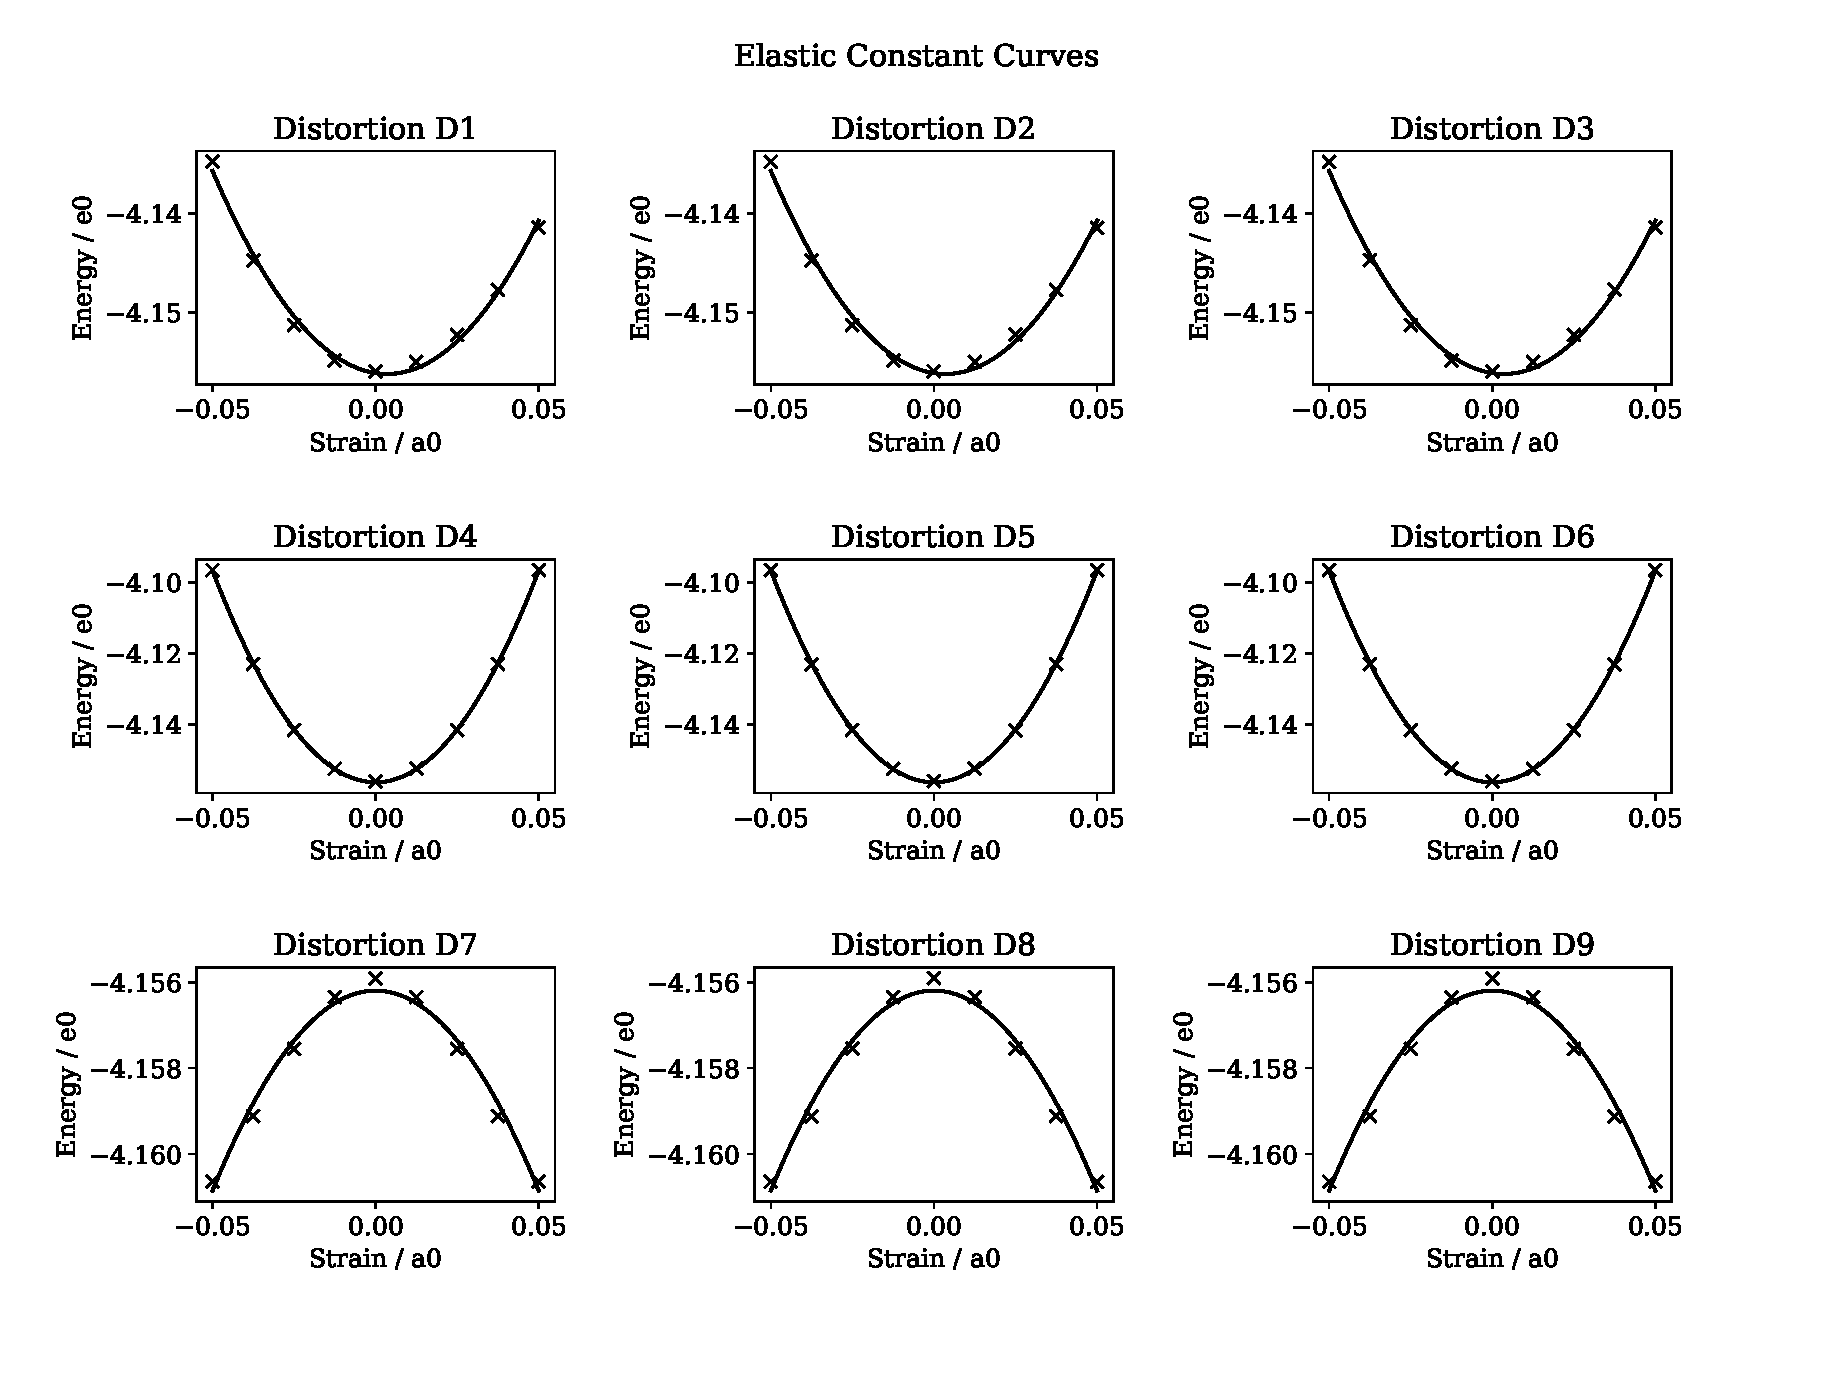
\includegraphics[width=.90\linewidth]{chapters/potentials_fe_pd_ru/fepd_potential/ec_rfkj/elastic_strains_bp_0.eps}  
\label{fig:fepd-fefcc-distortions}
\caption{Ravindran et al\cite{dfttisiravindran} distortion-energy plots for \acrshort{fcc} Pd}
\end{figure}

\begin{figure}[htb]
\begin{subfigure}{.42\textwidth}
  \centering
  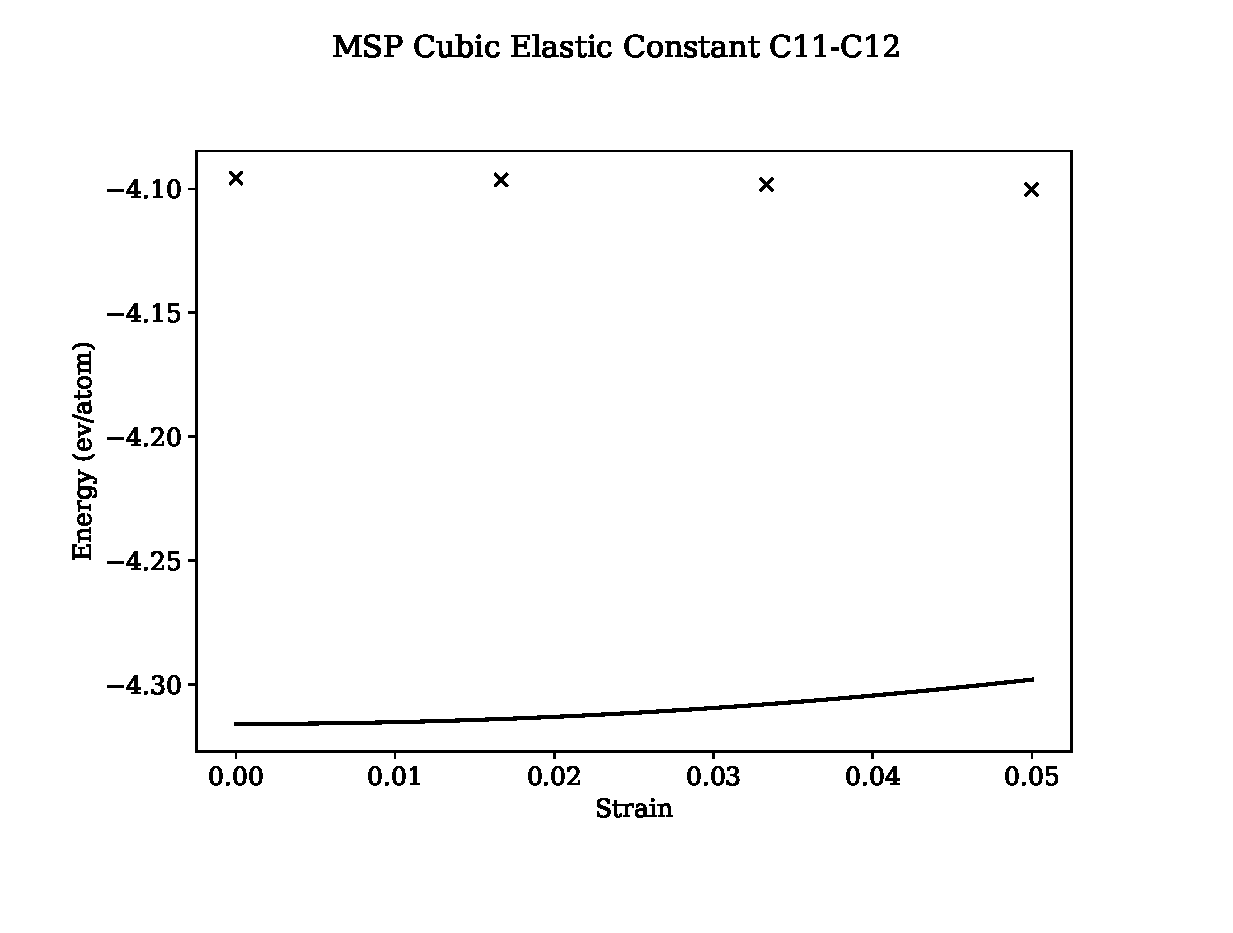
\includegraphics[width=.90\linewidth]{chapters/potentials_fe_pd_ru/fepd_potential/ec_mskp/msp_c11_c12_plot_bp_0.eps}  
  \caption{C11-C12 orthorhombic distortion}
  \label{fig:fepd-fefcc-c11c12}
\end{subfigure}
\begin{subfigure}{.42\textwidth}
  \centering
  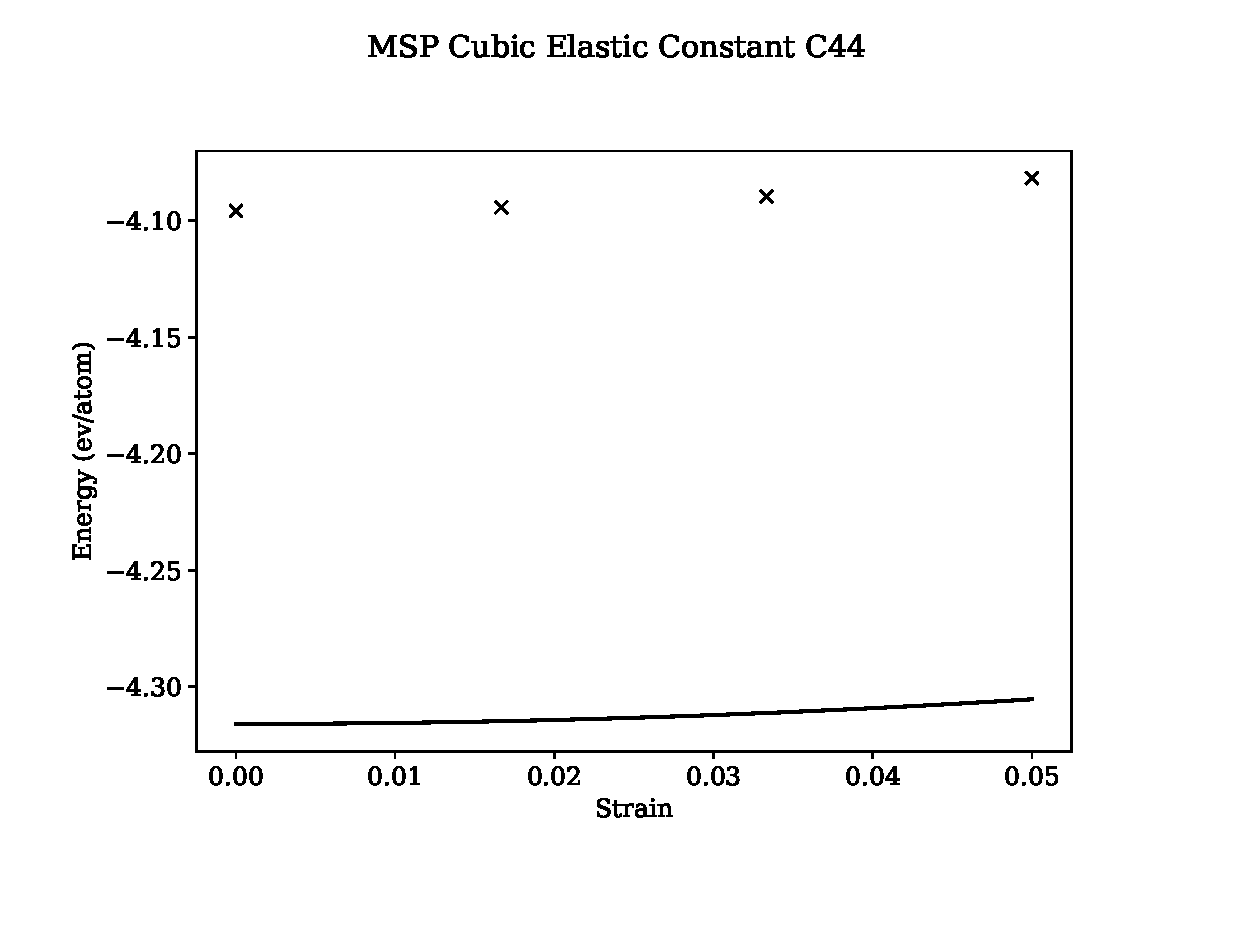
\includegraphics[width=.90\linewidth]{chapters/potentials_fe_pd_ru/fepd_potential/ec_mskp/msp_c44_plot_bp_0.eps}  
  \caption{C44 monoclinic distortion}
  \label{fig:fepd-fefcc-c44}
\end{subfigure}
\label{fig:feru-fefcc-c11c12c44}
\caption{Equation of State plots from this potential for \acrshort{fcc} Pd}
\end{figure}







